\chapter{Introduzione alla topologia generale}


Perché studiare topologia? \\
Oltre al fatto che sia (seppur discutibilmente) molto interessante e divertente, la topologia generalizza gli assiomi degli spazi metrici. \\ \\ 
Solitamente abbiamo visto in analisi - e vedremo anche più avanti - il caso degli intorni in formulazione \textit{epsilon-delta}, cioè le \textit{palle aperte}. Questa generalizzazione ci permette di estendere delle \enquote{buone} caratteristiche ad oggetti (o insiemi) che altrimenti non le avrebbero; alla fine del corso risulterà ovvio allora che gli spazi dell'analisi matematica fanno parte di una classe particolarmente privilegiata, sono più eccezione che norma. \\ \\ In un mondo regolato dal caos, non tutto può essere \enquote{bello e metrico}. La topologia ci permetterà di compiere un viaggio tra gli spazi più magnifici e perversi che la mente umana possa concepire, e vedremo che a volte persino concepirli sarà un bel problema. \\ \\
Insomma, che cosa aspettiamo?



\newpage
\section{La struttura di topologia}
\subsection{\textcolor{TopGener}{\textbf{Alcune definizioni fondamentali}}}

\begin{definition}
	Sia $X \neq \varnothing$. Una \textbf{struttura topologica su $X$}, o semplicemente topologia su $X$ (o di $X$), è una famiglia $\tau\subset 2^X$ di sottoinsiemi  che soddisfa le seguenti proprietà
	\begin{enumerate}
		\item $\varnothing, X \in \tau$
		\item $\tau$ è stabile per unione arbitraria, ovvero 
		\begin{equation*}
			\bigcup_{i \in I} A_i \in \tau 	
		\end{equation*}
		dove $I$ è un qualsiasi insieme indicizzante e $\forall i$ si ha che $A_i \in \tau$.
		\item $\tau$ è stabile per intersezioni finite, ovvero 
		\begin{equation*}
			\bigcap^n_{i=1} A_i \in \tau
		\end{equation*}
		dove $\forall i. \; A_i \in \tau$.
	\end{enumerate} 
\end{definition}

\begin{remark}
	È ovvio che l'ultima condizione si può riscrivere come: 
	\begin{center}
		$\forall \ A_1, A_2 \in \tau$ allora $A_1 \cap A_2 \in \tau$ 
	\end{center}
	Infatti per induzione si può ottenere di nuovo il terzo assioma. 
\end{remark}

\begin{definition}
	Sia $\tau$ una topologia su $X$, la coppia $(X, \tau)$ si chiama \textbf{spazio topologico}. $X$ è detto \textbf{supporto dello spazio topologico}. \\ Sia $A \in \tau$, $A$ è detto \textbf{sottoinsieme aperto di $(X,\tau)$} o aperto di $\tau$ oppure aperto di $X$ (se $\tau$ è implicitamente definita). 	
\end{definition}


Di seguito mostreremo come alcune semplici topologie possano essere collegate alla struttura di uno spazio metrico in modo più preciso; le due definizioni sono strettamente correlate anche in casi molto complessi, ma non ci estenderemo a tanto.

\begin{definition}
	Uno spazio topologico $(X,\tau)$ si dice \textbf{metrizzabile} se esiste una funzione distanza $\morphism{d}{X\times X}{\R}$ tale che gli insiemi aperti indotti da $d$ sono gli stessi elementi di $\tau$. \\ In particolare se uno spazio è metrizzabile allora la topologia indotta da $d$ è la stessa già presente nello spazio, $\tau_d  = \tau$. 
\end{definition}

Di seguito mostreremo come alcune semplici topologie possano essere collegate alla struttura di uno spazio metrico in modo più preciso; le due definizioni sono strettamente correlate anche in casi molto complessi, ma non li studieremo in modo approfondito. Parlando di un caso davvero banale, diciamo \textbf{topologia euclidea} la topologia su $\mathbb{R}^n$ associata alla ben nota \textit{distanza euclidea}. Già al nostro marginale livello di trattazione, il caso euclideo (e quindi campo dell'analisi matematica) risulta essere una \enquote{banale} eccezione.
\\ \\ Questo è esattamente ciò di cui stavamo parlando, il fatto che uno spazio ammetta una funzione distanza compatibile con la propria topologia non è affatto scontato; o almeno non lo è nella maggior parte delle volte. \\ Altri spazi più \textit{patologici} sono metrizzabili, e questo induce su di loro la struttura di spazio metrico. \\ Notiamo un fatto importante, che dovrebbe essere ovvio ma è bene sottolineare. Se uno spazio è metrizzabile, quindi se la sua topologia è compatibile con una funzione distanza $d$, allora gli aperti possono essere costruiti come unione di $B_d(x_i,r_i)$ per $r_i \in \mathbb{R}$, $x_i \in \mathbb{R}$. Vedremo in seguito che questi costituiscono una \textit{base della topologia}, ma diamo tempo al tempo.
\begin{example}\
\begin{enumerate}
	\item Sia $(X,d)$ uno spazio metrico e sia la famiglia $\tau_d$ degli aperti di $X$ rispetto a $d$. Allora $(X,\tau_d)$ formano uno spazio topologico. 
	\item La topologia più povera in assoluto è la \textit{topologia banale}: 
	\begin{center}
		$\tau = \left\{\varnothing, X\right\}$ 
	\end{center}
	Vediamo che non è metrizzabile se non nel caso in cui $X = \left\{x\right\}$, ovvero quando $X$ è un \textit{singoletto}. \\ Infatti sia $d$ una distanza su $X$ e sia $X = \left\{p,q\right\}$ allora per ogni $\rho > 0$ si ha che $q \in B_\rho(p)$, quindi $d(p,q) = 0$. Ma poiché $d$ è una distanza ottengo che $p=q$, contraddicendo l'ipotesi $p \neq q$. \\ Nel caso del singoletto invece è elementare che sia metrizzabile.
	\item Dall'altra parte della barricata c'è la \textit{topologia discreta}: 
	\begin{center}
		$\tau = 2^X$
	\end{center}
	Questa è la più ricca topologia possibile da indurre su un insieme; infatti se $\tau$ è una topologia ho che $\tau \subseteq 2^X$. \\ Si tratta ovviamente di una topologia (la verifica è immediata) e vale anche l'assioma della stabilità per intersezioni di famiglie arbitrarie. \\ Inoltre è sempre metrizzabile per ogni $X \neq \varnothing$: infatti basta prendere la distanza $d(x,y) = 1$ se $x \neq y$, $0$ altrimenti. \footnote{si può anche prendere un valore arbitrario, come $69.42^{0.314159}$; non è questo il punto.}
	\item Definiamo la \textit{topologia cofinita} come segue:
	\begin{equation*}
		\tau_{\text{cof}} \coloneqq \left\{\varnothing\right\} \cup \left\{ A \in 2^X  \,\middle|\, A^c\ \text{è finito}\ \right\}
	\end{equation*}
	Si dimostra che è una topologia.
	\begin{enumerate}
		\item $\varnothing \in \tau_{cof}$. Inoltre $X^c = \varnothing$ e $\varnothing$ è ovviamente finito. Quindi $X \in \tau_{cof}$.
		\item Dimostro la stabilità per unione di famiglie arbitrarie di $\tau_{cof}$. \\ Siano $C_i$ i complementari finiti di $A_i$ per ogni $i$.
			\begin{equation*}
					\bigcup_{i \in I} A_i = \bigcup_{i \in I} C_i^c = \left(\bigcap_{i \in I} C_i\right)^c \subseteq C_j
			\end{equation*}
		per qualunque insieme $I$ e qualche $j \in I$. Per cui visto che $A_j \in \tau_{\text{cof}}$ risulta che $C_j$ sia finito.
		\item Siano $A_1, A_2 \in \tau_{\text{cof}}$, allora $(A_1 \cap A_2)^c = A^c_1 \cup A^c_2$ e l'unione finita di insiemi finiti è finito, per cui anche $A_1 \cap A_2 \in \tau_{\text{cof}}$. 
	\end{enumerate}	
	Inoltre non è metrizzabile perché se lo fosse sarebbe di Hausdorff, ma come si vedrà, non è di Hausdorff; quindi non può neppure essere metrizzabile.
\end{enumerate}
\end{example}



\subsection{\textcolor{TopGener}{\textbf{Confronto tra topologie}}}

Risulta perfettamente naturale chiedersi quando due topologie siano \enquote{uguali}, o comunque \enquote{confrontabili}. Ma come si definisce per una topologia l'essere \enquote{uguale} ad un'altra? In che senso una topologia è \enquote{paragonabile} ad un'altra? \\ \\ Intuitivamente vogliamo lavorare sulla struttura topologica che inducono nello spazio, ma questa intuizione deve essere formalizzata.



\begin{definition}
	Sia $X \neq \varnothing$. Siano $\tau, \tau'$ due topologie su $X$. Diciamo che $\tau$ è \textbf{meno fine} (più fine) di $\tau'$ se $\tau \subset \tau'$ ($\tau' \subset \tau$).
\end{definition}

\begin{definition}
	Due topologie $\tau, \tau'$ si dicono \textbf{confrontabili} se $\tau$ è più fine o meno fine o uguale a $\tau'$. \\ Evidentemente, non tutte le topologie sono confrontabili tra loro.
\end{definition}

\begin{example}
	Alcuni esempi di confronto tra topologie.
	\begin{enumerate}
		\item La topologia banale è la meno fine di tutte le topologie di $X$.
		\item La topologia discreta è la più fine delle topologie su $X$.
		\item Sia $X = \left\{a,b\right\}$, allora $\tau = \left\{\varnothing,\left\{a\right\}, X\right\}$ e $\tau' = \left\{\varnothing, \left\{b\right\}, X\right\}$ sono topologie non confrontabili.
	\end{enumerate}
\end{example}



\newpage
\section{Basi e sottobasi di topologie}
\subsection{\textcolor{TopGener}{\textbf{Semplificare la scrittura: basi di topologie}}}



Poiché le topologie possono essere molto complesse, sarebbe utile avere un modo per poterle scrivere (o costruire) più semplicemente. \\ Scegliamo il seguente approccio: cerchiamo una sottofamiglia $B$ della topologia tale che ogni $A$ elemento della topologia si possa scrivere come unione di insiemi $B_j$ contenuti in $B$; intuitivamente sarà un po' come i generatori per i gruppi o le basi per gli spazi vettoriali. \\ Vediamo come costruire le \textit{basi di una topologia}.

\begin{definition}
	Sia $X \neq \varnothing$. $(X, \tau)$ spazio topologico e sia $\mathcal{B} \subset \tau$. \\ $\mathcal{B}$ è una \textbf{base di $\tau$} se $\forall A \in \tau \ \exists \left\{B_i\right\}_{i \in I} \subset \mathcal{B}$ per cui $\bigcup_{i \in I} B_i = A$. \\ O analogamente se la definisco come segue:
	\begin{equation*}	
		\tau \coloneqq \left\{A \in 2^X \,\middle|\, \exists \mathcal{B}' \subset \mathcal{B} , \; \bigcup_{B \in \mathcal{B}'} B = A \right\}
	\end{equation*}
\end{definition}

\begin{proposition}
	$\mathcal{B}$ è una base se e solo se 
	\begin{equation*}
	\forall A \in \tau\ \forall x \in A\ \exists B \in \mathcal{B} \ \text{ tale che } \ x \in B \subset A
	\end{equation*}
\end{proposition}
\begin{proof} Dimostriamo che valgono entrambe le implicazioni:
	\begin{enumerate}
		\item[($\Rightarrow$)] Scelgo un $x \in A$, poiché $\mathcal{B}$ è una base $A = \bigcup_{B \in \mathcal{B}'} B$. \\ Riscrivendo ottengo $x \in A = \bigcup_{B \in \mathcal{B}'} B$, di conseguenza esiste almeno un $B \in \mathcal{B}' \subset \mathcal{B}$ per cui $x \in B$.
		\item[($\Leftarrow$)]  Sia $A \in \tau$, allora posso prendere ogni $x \in A$ e avere che $x \in B_x$ per qualche $B_x \in \mathcal{B}$. Inoltre $B_x \subset A$ per ogni $x \in A$, quindi devo dimostrare che $A \subset \bigcup_{x \in A} B_x$, ma ciò è banalmente vero. \footnote{(sia $x \in A$, allora $x \in B_x \subset \bigcup_{x \in A} B_x$).}
	\end{enumerate}
\end{proof}

\begin{example}
	Alcuni esempi istruttivi nella loro semplicità.
	\begin{enumerate}
		\item Dato uno spazio topologico $(X,\tau)$, $\tau$ è una base di $\tau$. 
		\item Se $\mathcal{B}$ è una base di $\tau$, allora sia $\mathcal{B} \subset C$, allora anche $C$ è una base di $\tau$.
		\item In $\R$ una base può essere $\mathcal{B} = \left\{(a,b) \,\middle|\, a,b \in \R, \; a < b \right\}$
	\end{enumerate}
\end{example}

\begin{proposition}
	Sia $X \neq \varnothing$ e $\left\{\tau_i\right\}$ una famiglia di topologie su $X$. \\ Valgono i seguenti enunciati:
	\begin{enumerate} 
		\item $\tau_\cap = \bigcap_{i \in I} \tau_i$ è una topologia di X.
		\item L'unione di topologie non è sempre una topologia.
		\item Sia dato un insieme $\mathcal{Y} \subset 2^X$, sia $\{\tau_i\}_{i \in I}$ una famiglia di insiemi di $X$ presa come segue
		\begin{equation*}
			\mathcal{Y} \subset \tau_i \; \forall i \in I
		\end{equation*}
		allora 
		\begin{equation*}
			\tau_\cap \coloneqq \bigcap_{i \in I} \tau_i	
		\end{equation*}
		 è la topologia meno fine su $X$ tale da contenere $\mathcal{Y}$.
	\end{enumerate}
\end{proposition}
\begin{proof} \
	\begin{enumerate}
		\item $\varnothing, X \in \tau_\cap$, poi l'unione e l'intersezione vengono per il fatto che sono elementi di qualche topologia.
		\item Controesempio alla tesi che l'unione di topologie è ancora una topologia. Sia $X = \left\{a,b,c\right\}$ allora definisco $\tau = \left\{\varnothing, \left\{a,b\right\}, X\right\}$ e $\tau' = \left\{\varnothing, \left\{b,c\right\}, X\right\}$, l'unione non contiene $b$, ma $\left\{a,b\right\} \cap \left\{b,c\right\} = \left\{b\right\}$ per cui l'unione delle topologie non è una topologia.
		\item Per il primo punto $\bigcap_{i \in I} \tau_i$ è una topologia, e contiene $\mathcal{Y}$ per definizione. \\ Dimostro che è la meno fine. Infatti sia $\tau' \subset \bigcap_{i \in I} \tau_i$ e per cui $\tau' \subset \mathcal{Y}$, allora $\tau' \in \left\{\tau_i\right\}$ e quindi $\bigcap_{i \in I} \tau_i \subset \tau'$. 
	\end{enumerate}	
\end{proof}

\begin{remark}
	Sia $(X, \tau)$ uno spazio topologico la cui base è $\mathcal{B}$, allora valgono le seguenti proprietà:
	\begin{enumerate}
		\item $\bigcup_{B \in \mathcal{B}'} B = X$ per qualche sottofamiglia $\mathcal{B}' \subset \mathcal{B}$. 
		\footnote{Vale banalmente, visto che $X \in \tau$ per la definizione di base segue che $\mathcal{B}$ è un ricoprimento di $X$.}
		\item Se $B_1, B_2 \in \mathcal{B}$ allora $B_1 \cap B_2 \in \tau$, quindi per la definizione di base segue che $B_1 \cap B_2  = \bigcup_{B \in \mathcal{B}'} B$ per qualche $\mathcal{B}' \subset \mathcal{B}$.
		\item Il punto precedente vale $\forall B_1, B_2 \in \mathcal{B}$; allora se $B_1 \cap B_2 \neq \varnothing$ abbiamo che $\forall x \in B_1 \cap B_2$ esiste $B_x \in \mathcal{B}$ tale che $x \in B_x \subset B_1 \cap B_2$.
	\end{enumerate}
\end{remark}

\begin{theorem}
	\label{thr:set_simil_base_generate_top}
	Sia $X \neq \varnothing$ e sia $\mathcal{B}$ una famiglia di sottoinsiemi di $X$. \\ Supponendo che 
	\begin{enumerate}
		\item $\mathcal{B}$ è un ricoprimento di $X$.
		\item Sono dati $A_1, A_2 \in \mathcal{B}$ con $A_1 \cap A_2 = \bigcup_{B \in \mathcal{B}} B$  
	\end{enumerate}
	Allora $\mathcal{B}$ è una delle basi di una topologia $\tau_\mathcal{B}$ su $X$; in particolare è l'unica definita da $\mathcal{B}$ ed è la meno fine che contiene $\mathcal{B}$.
\end{theorem}
\begin{proof}
	Se $\tau$ esiste è unica. Infatti dovendo $\mathcal{B}$ essere una sua base allora per definizione di base 
	\begin{equation*}	
		\tau \coloneqq \left\{A \in 2^X \,\middle|\, \exists \mathcal{B}' \subset \mathcal{B} , \; \bigcup_{B \in \mathcal{B}'} B = A \right\}
	\end{equation*}
	Inoltre se esiste è la più piccola contenente $\mathcal{B}$.
	Per cui dimostro che $\tau$ è una topologia e la dimostrazione è finita.
	\begin{enumerate}
		\item $\varnothing, X \in \tau$ poiché $\mathcal{B}$ è un ricoprimento di $X$ e inoltre anche $\varnothing \in \tau$ perché basta prendere la sottofamiglia vuota di $\mathcal{B}$ per ottenerlo.
		\item L'unione di sottofamiglie di $\mathcal{B}$ è l'unione di elementi di $\mathcal{B}$ poiché ogni elemento in $\tau$ è unione di elementi in $\mathcal{B}$.
		\item Analogamente per l'intersezione, dove basta aggiungere l'osservazione che 
		\begin{align*}
			A_1 \cap A_2 & = \bigcup_{i} B_{1,i} \cap \bigcup_{j} B_{2,j} \\
				& = \bigcup_{i,j} B_{1,i} \cap B_{2,j} =\bigcup_{k} B_{k}
		\end{align*}
		per un $k \in I_{i,j}$ insieme degli indici dipendente da $i$ e $j$. \\ Ovvero è ancora contenuto in $\tau$, visto che basta prendere l'unione di una sottofamiglia di $\mathcal{B}$.
	\end{enumerate}
\end{proof}


\newpage
\subsection{\textcolor{TopGener}{\textbf{La sottobase di una topologia}}}



L'idea dietro la costruzione di una sottobase è mostrare un modo semplice di costruire le basi di topologie, che abbiamo visto non essere sempre amichevoli. Spesso ostili, queste possono essere scritte agilmente grazie a quanto vedremo.

\begin{definition}
	Sia $(X,\tau)$ uno spazio topologico e sia $S \subset \tau$. Si dice che $S$ è una \textbf{sottobase di $\tau$} se genera gli elementi di una base $\mathcal{B}$ tramite di intersezioni finite. La base generata da $S$ si definisce nel seguente modo 
	\begin{equation*}
		 \mathcal{B} = \langle S\rangle \coloneqq \left\{ B \in 2^X \,\middle|\, \bigcap_{i \in I} S_i = B \, \text{ per un indice con } |I| < +\infty \right\}
	\end{equation*}
	.
\end{definition}

\begin{example}\
\begin{enumerate}
	\item $S = \tau$ è una sottobase, inutile, ma lo è.
	\item Si prenda la topologia $2^X$ dove $X = \left\{a,b,c\right\}$, allora $S = \left\{\left\{a,b\right\},\left\{a,c\right\},\left\{c,b\right\}\right\}$ è una sottobase di $\tau$.
	\item Si consideri $\R$, una sua sottobase potrebbe essere $S \coloneqq \left\{(-\infty, a) \,\middle|\, a \in \R\right\} \cup \left\{(b, +\infty) \,\middle|\, b \in \R\right\}$
\end{enumerate}
\end{example}

\begin{proposition}
	$\mathcal{S}$ è una sottobase di $\tau$ se e solo se
	\begin{equation*}
	\forall \ A \in \tau \; . \forall x \in A . \; \exists \ U_1, \dots, U_n \in \mathcal{S} \ \text{ tali che } \ x \in U_1 \cap \dots \cap U_n \subset A
	\end{equation*}
\end{proposition}
\begin{proof}
	Riesce immediatamente, usa le definizioni locali di base ricordandoti che la sottobase definisce una base.
\end{proof}

\begin{remark}
	Nella proposizione precedente abbiamo ricavato una definizione equivalente di sottobase; usiamo questa definizione con al posto di $A$ tutto l'insieme $X$, si ha immediatamente che $\mathcal{S}$ forma un ricoprimento di $X$.
\end{remark}

\begin{proposition}
	Se $\mathcal{S} \subset 2^X$ è un ricoprimento di $X$ allora $\mathcal{S}$ è una sottobase di $(X,\tau)$, ed esiste un'unica topologia su $X$ con questa sottobase generatrice della base. \\ Quindi $\tau$ è l'unica topologia generata da $\mathcal{S}$, ed in particolare è anche la meno fine tra tutte le generabili da $\mathcal{S}$.
\end{proposition}
\begin{proof}
	Se si prova l'esistenza della topologia allora è l'unica ed è anche la più fine.
	Perciò per il Teorema \ref{thr:set_simil_base_generate_top} basta dimostrare che la base $\mathcal{B}$ generata da $\mathcal{S}$ è tale da essere un ricoprimento e che l'intersezione finita di elementi di $\mathcal{B}$ è stabile.\\
	Come base usiamo ovviamente
	\begin{equation*}
	\mathcal{B} = \left\{ A \in 2^X \ \Big|\ \exists \ U_1, \dots, U_n \in \mathcal{S} \ \text{ con } A = \bigcap_{i } U_i \right\}
	\end{equation*}
	\begin{enumerate}
		\item Per ipotesi $\mathcal{S}$ è un ricoprimento e $\mathcal{S} \subset \mathcal{B}$ quindi anche $\mathcal{B}$ è ovviamente un ricoprimento di $X$.
		\item Siano $B_1, B_2 \in \mathcal{B}$ allora sono intersezione finita di elementi di $\mathcal{S}$ per cui
		\begin{equation*}
			B_1 \cap B_2 = \bigcap^n_{i=1} U_i \cap \bigcap^{m}_{j=1} U_j = \bigcap^{n+m}_{i=1} U_i  \in \mathcal{B}
		\end{equation*}
	\end{enumerate}
	quindi utilizzando il Teorema \ref{thr:set_simil_base_generate_top} si conclude.
	\end{proof}

\begin{remark}
	Se $\mathcal{S} = \left\{X\right\}$ è ovvio che $\mathcal{B} = \left\{\varnothing, X\right\}$, poiché $\varnothing = \bigcup_{A \in \mathcal{A}} A $ dove $\mathcal{A}$ è la famiglia vuota. \\ Quindi $\mathcal{S}$ induce la topologia banale, che è la meno fine in assoluto.
\end{remark}



\newpage
\section{Intorni e sistemi fondamentali di intorni}
Ad un certo punto, nello studio di analisi si è destinati ad incontrare gli \textit{intorni}. \\ L'idea alla base dello studio della topologia è ampliare e generalizzare quanto è possibile fare con la \enquote{banale} analisi matematica in $\mathbb{R}^n$, quindi è più che naturale arrivare a trattare di intorni. \\ \\ In analisi matematica si definiscono con la formulazione detta \textit{epsilon-delta}, e sono solitamente intorni circolari (nel caso $n=2$); vedremo in questo capitolo un modo per rendere più generali tali definizioni e strutture, oltre all'importanza che ricopriranno nel corso delle dimostrazioni e della teoria di topologia generale, ma anche di algebra e di gran parte della matematica.


\subsection{\textcolor{TopGener}{\textbf{Gli intorni in topologia}}}




\begin{definition}
	Sia $(X,\tau)$ uno spazio topologico e sia $M \in 2^X$. Un sottoinsieme $U \subset X$ si dice \textbf{intorno di $M$ in $(X,\tau)$} se esiste un aperto $A$ tale che $M \subset A \subset U$. \\ \\ In particolare se $M$ è un insieme singoletto si può semplificare la scrittura a $M = \left\{m\right\}$, quindi $U$ è un intorno di $x$ in $(X,\tau)$ se esiste un aperto $A$ tale che $x \in A \subset U$.
\end{definition}

\begin{definition}
	Indichiamo con $\mathcal{N}_\tau(x)$ l'insieme degli intorni di $x$ in $(X,\tau)$. 
	\begin{equation*}
		\mathcal{N}_\tau(x) \coloneqq \left\{ U \in 2^X \,\middle|\, \exists A \in \tau\ .\ x \in A \subset U \right\}
	\end{equation*}
	In particolare $\mathcal{N}_\tau(x)$ si dice \textbf{sistema di intorni} di $x$ in $(X, \tau)$.
\end{definition}

\begin{remark} \
	\label{rmk:intorni_top}
	\begin{enumerate}
		\item Se $U \in \mathcal{N}_\tau(x)$ allora $x \in U$.
		\item $\forall A \in \mathcal{N}_\tau(x) \; \exists C \in \mathcal{N}_\tau(x)$ tale che $C \subset A$ e $C$ aperto. Ovvero a meno di restrizioni ogni intorno è aperto, questo è ovvio dalla definizione (basta prendere l'aperto $C$ che rende $A$ intorno di $x$ con $x\in C \subset A$).
		\item Se $U \in \mathcal{N}_\tau(x)$ e prendo $V \in 2^X$ tale che $U \subset V$ allora ottengo che $V \in \mathcal{N}_\tau(x)$. 
	\end{enumerate}	
\end{remark}

\begin{proposition}
	Sia $(X,\tau)$ uno spazio topologico, e sia $A \in 2^X$. \\ Allora $A \in \tau$ se e solo se $\forall x \in A . \; A \in \mathcal{N}_\tau(x)$. \\ Oppure,  equivalentemente, se $A \in \bigcap_{x \in A} \mathcal{N}_\tau(x)$.
\end{proposition}
\begin{proof} \
	\begin{enumerate}
		\item[$(\Rightarrow)$] La prima implicazione è ovvia poiché $A$ aperto. Allora $x \in A \subset A$ per ogni $x \in A$.
		\item[$(\Leftarrow)$]	La seconda pure perché $A$ è un intorno di ogni suo punto, e quindi esiste $x \in A_x \subset A$ tale che $A_x \in \tau$. Allora
		\begin{equation*}
			A = \bigcup_{x \in A} \left\{x\right\} \subset \bigcup_{x\in A} A_x \subset A
		\end{equation*}
		da cui $A \in \tau$ perché unione di aperti. 
	\end{enumerate}
\end{proof}

Dalle osservazioni che seguono vedremo come una topologia induce sugli intorni certe proprietà, ma allo stesso modo se si danno quelle proprietà a degli intorni questi creano una topologia. Insomma, una topologia genera degli intorni se e solo se quegli stessi intorni generano la suddetta topologia. Questo è dato dal fatto che esistono diverse definizioni equivalenti di topologia, tra le quali esiste quella per filtri e filtri principali (si veda \url{https://leanprover-community.github.io/theories/topology.html}). \\
A meno di restrizioni, ogni intorno appartenente al sistema di intorni è aperto (basti pensare alla definizione di intorno, con $x \in U \subset A$ ed $U \in \tau$, bisogna solo eventualmente restringersi all'aperto $A$). Gli intorni quindi possono sostituirsi agli aperti, ma sotto opportune condizioni.

\begin{proposition}
	Sia $(X,\tau)$ uno spazio topologico ed $x \in X$, indichiamo per semplicità $\mathcal{N}_\tau(x) = \mathcal{N}(x)$. Valgono le seguenti proprietà:
	\begin{enumerate}
		\item Se $U \in \mathcal{N}_\tau(x)$ e $V \in 2^X$ tale che $U \subset V$, allora $V \in \mathcal{N}_\tau(x)$
		\item Siano $N_i \in \mathcal{N}(x)$, allora 
		\begin{equation*}
			\bigcap^{n}_{i=0} N_i \in \mathcal{N}(x)
		\end{equation*}
		\item Se $U \in \mathcal{N}_\tau(x)$, $x \in U$. 
		\item Se $U \in \mathcal{N}(x) \ \exists V\ .\ V \subset U$ tale che $V \in \mathcal{N}(x)$ e $\forall y \in V\ .\ U \in \mathcal{N}(y)$.
	\end{enumerate}
\end{proposition}
\begin{proof} \
	\begin{enumerate}
		\item Si veda l'Osservazione \ref{rmk:intorni_top}.
		\item Basta far vedere che $N_1 \cap N_2 \in \mathcal{N}(x)$, il ché è ovvio. \\ Per definizione di intorno 
			esistono $A_1, A_2 \in \tau$ tali che $A_1 \subset N_1$ e $A_2 \subset N_2$, per cui $x \in A_1 \cap A_2 \subset N_1 \cap 
			N_2$; e per definizione di aperti $A_1 \cap A_2$ è aperto.  La definizione di intorno è soddisfatta, 
			$N_1 \cap N_2 \in \mathcal{N}(x)$.
		\item Si veda l'Osservazione \ref{rmk:intorni_top}.
		\item Si scelga $V = A$ dove $A \subset U$ e $A \in \tau$. Per la definizione di intorno, $A$ esiste e soddisfa la proprietà richiesta. 
	\end{enumerate}
\end{proof}  

\begin{proposition}
	Sia $X \neq \varnothing$ e ad ogni $x \in X$ sia associata la famiglia di intorni $\mathcal{N}(x)$, ovvero la famiglia che possiede le seguenti proprietà:
	\begin{enumerate}
		\item Se $U \in \mathcal{N}_\tau(x)$ e $V \in 2^X$ tale che $U \subset V$ allora $V \in \mathcal{N}_\tau(x)$
		\item Siano $N_i \in \mathcal{N}(x)$, allora 
			\begin{equation*}
				\bigcap^{n}_{i=0} N_i \in \mathcal{N}(x)
			\end{equation*}
		\item Se $U \in \mathcal{N}_\tau(x)$, $x \in U$. 
		\item Se $U \in \mathcal{N}(x) \exists V .\ V \subset U$ 
			tale che $V \in \mathcal{N}(x)$ e $\forall y \in V.\ U \in \mathcal{N}(y)$.
	\end{enumerate}
	Allora esiste una ed un'unica topologia $\tau$ tale che $\forall x \in X .\ \mathcal{N}(x) = \mathcal{N}_\tau(x)$.
\end{proposition}
\begin{proof}
	Definiamo innanzitutto una topologia come segue (il che richiede la presenza dell'ipotesi $3$)
	\begin{equation*}
		\tau \coloneqq \left\{ A \in 2^X \,\middle|\, \forall x \in A\ . \ \exists N \in \mathcal{N}(x)\ \text{t.c.}\ x \in N \subset A \right\}
	\end{equation*}
	Mostriamo la sua struttura topologica:
	\begin{enumerate}
		\item $\varnothing \in \tau$ in quanto non avendo punti soddisfa il criterio, mentre $X \in \tau$ dato che per il punto $1$ ho che $U \subset X$ per ogni $U \in \mathcal{N}(x)$ ($x \in X$ qualsiasi).
		\item Mostro che se $A_1, A_2 \in \tau$ allora $A_1 \cap A_2 \in \tau$. \\ Sia $x \in A_1 \cap A_2$, per definizione di $A_1$ deve esistere almeno un insieme $U \in \mathcal{N}(x)$ tale che $U \subset A_1$, e lo stesso vale per $V \subset A_2$. Quindi prendo $V \cap U \subset A_1 \cap A_2$ e per il punto $2$ deve essere $U \cap V \in \mathcal{N}(x)$. \\ Quindi $A_1 \cap A_2 \in \tau$.
		\item Devo dimostrare che rimane stabile per unione arbitraria di aperti. \\ Considero una famiglia $\left\{A_i\right\}_{i \in I}$ con $I$ insieme qualunque. Denominiamo poi $S = \bigcup_{i \in I} A_i$. Per cui sia $x \in S$, allora deve esistere $x \in A_{i_0}$. Per definizione di aperto deve esistere $U\in \mathcal{N}(x)$ tale che $x \in U \subset A_{i_0}$. Poiché questo vale per ogni $x \in S$ segue che
		\begin{equation*}
			\bigcup_{i \in I} U_i \subset  S = \bigcup_{x \in S} \left\{x\right\} = \bigcup_{i \in I} A_i 
		\end{equation*}
		e l'unione degli $U_{i_0} \subset \bigcup_{i \in I} U_i$. 
		\footnote{per l'ipotesi $4$ posso trovare un ricoprimento di $U_i \in \mathcal{N}(y)$ per ogni $y \in A_i$!}
		\\
		 Quindi per la definizione della topologia segue che l'unione di questi intorni è ancora un intorno di ogni punto di $S$. Pertanto $S \in \tau$.
	\end{enumerate}
	Per come si possono caratterizzare gli insiemi aperti, ovvero come intorni di ogni loro punto, dev'essere che la topologia sopra definita sia l'unica.  
\end{proof}



\subsection{\textcolor{TopGener}{\textbf{Sistemi fondamentali di intorni}}}



Gli intorni sono tanti. \textit{Davvero} tanti. \\ Fatto sta che spesso e volentieri sono infiniti; incontriamo lo stesso problema delle topologie. Come possiamo descrivere un sistema di intorni in modo computabile entro la fine dell'universo? \\ Qui entrano in gioco i sistemi fondamentali di intorni.


\begin{definition}
	Sia data una famiglia $\mathcal{V}(x)$ di intorni di $x$ in $(X,\tau)$, cioè una famiglia $\mathcal{V}(x) \subset \mathcal{N}_\tau(x)$; questa si dice \textbf{sistema fondamentale di intorni} di $x$ in $(X,\tau)$ se $\forall U \in \mathcal{N}_\tau(x)\ .\ \exists V \in \mathcal{V}(x)$ tale che $V \subset U$.
\end{definition}

\begin{example} Esempi di sistemi fondamentali di intorni:
\begin{enumerate} 
	\item Sia $(X,\tau)$ spazio topologico metrizzabile tramite una distanza $d$. Possiamo definire $\mathcal{V}(x) = \left\{B_d(x,r)\right\}_{r>0}$ come sistema fondamentale di intorni di $x$. 
	\item Sia $(X,\tau)$ con $\tau$ topologia banale e $x \in X$; l'unica scelta come intorno è $X$ stesso, quindi $V(x) = \left\{X\right\}$.
	\item Sia $(X,\tau)$ con $\tau$ topologia discreta e $x \in X$, basta prendere $\mathcal{V}(x) = \left\{\left\{x\right\}\right\}$ come sistema fondamentale di intorni.
\end{enumerate}
\end{example}

\begin{proposition}
	Sia $(X,\tau)$ uno spazio topologico $\forall x \in X$, sia $\mathcal{V}(x) \subset \mathcal{N}_\tau(x)$ tale che $\mathcal{V}(x)$ è un sistema fondamentale di intorni. Sia inoltre $A \in 2^X$. \\ Allora $A \in \tau$ se e solo se $\forall x \in A\ \exists V(x)$ tale che $V(x) \subset A$.
\end{proposition}
\begin{proof}
	Se $A$ è aperto allora è anche un intorno di $x \in A$. Per definizione di sistema fondamentale di intorni ottengo che esiste $V(x) \in \mathcal{V}(x)$ tale che $V(x) \subset A$.\\
	Se vale $\forall x \in A\ .\ \exists V(x) \in \mathcal{V}(x)$ tale che $V(x) \subset A$. 
	\begin{equation*}
		A = \bigcup_{x \in A} \left\{x\right\} \subset \bigcup_{x \in A} A_x \subset \bigcup_{x \in A} V(x) \subset A
	\end{equation*}
	Poiché $V(x)$ è un intorno di $x$, esiste $A_x$ aperto tale che $A_x \subset V(x)$.
\end{proof}

\begin{theorem}
	Sia $(X,\tau)$ spazio topologico e $\mathcal{B} \subset \tau$; allora $\mathcal{B}$ è una base per $\tau$ se e soltanto se $\forall x \in X$ la famiglia 
	\begin{equation*}
	\mathcal{B}(x) = \left\{B \in \mathcal{B} \,\middle|\, x \in B \right\}
	\end{equation*}
	è un sistema fondamentale di intorni di $x$ rispetto a $\tau$.
\end{theorem}
\begin{proof}
	Sia $\mathcal{B}$ una base di $\tau$ e $x \in X$. Sia $U \in \mathcal{N}_\tau(x)$, per definizione $\exists A \in \tau$ tale che $x \in A \subset U$. \\ Poiché $\mathcal{B}$ base di $\tau$, allora $A = \bigcup_{B \in \mathcal{B}'} B$ con $\mathcal{B}' \subset \mathcal{B}$. Perciò $x \in A$, che implica $x \in B$ per qualche $B \in \mathcal{B}' \subset \mathcal{B}$, ed otteniamo che $B \in \mathcal{B}(x)$. \\ Quindi dimostro che per ogni intorno $N(x) \in \mathcal{N}(x)$; segue che esiste $B \subset N(x)$, ovvio perché per definizione di intorno $x \in A \subset N(x)$, ma $A = \bigcup_{B \in \mathcal{B}'} B$ per qualche $\mathcal{B}' \subset \mathcal{B}$.\\  	
	Supponiamo che $\mathcal{B}(x)$ sia un sistema fondamentale di intorni per ogni $x \in X$. Sia $A \in \tau$, per la proposizione precedente allora $\forall x \in A, \exists V(x) \in \mathcal{B}(x)$ tale che $V(x) \subset A$. In particolare ottengo che
	\begin{equation*}
		A = \bigcup_{x \in A} \left\{x\right\} \subset \bigcup_{x \in A} V(x) \subset A
	\end{equation*} 
	poiché ogni $V(x) \subset A$ per definizione. Pertanto $\mathcal{B}(x)$ forma una base per tutti gli aperti in $\tau$.
\end{proof}

\begin{corollary}
	\label{crl:base_from_sfi}
	Sia $(X,\tau)$ spazio topologico. \\ Supponiamo che $\forall x \in X$, $\mathcal{V}(x) \subset \mathcal{N}_\tau(x) \cap \tau$. Allora 
	\begin{equation*}
		\mathcal{B} = \bigcup_{x \in X} \mathcal{V}(x) \subset \tau
	\end{equation*}
	ed è una base di $\tau$.
\end{corollary}
\begin{proof}
	Dalla definizione data di $\mathcal{B}$ sappiamo che $\forall x . \ \mathcal{V}(x) \subset \mathcal{B}$, e quindi $\mathcal{B}$ forma un sistema fondamentale di intorni. \\ Per il teorema precedente, $\mathcal{B}$ forma una base di $\tau$.
\end{proof}

\begin{remark}
	Sia $(X, \tau)$ uno spazio topologico tale che $\forall x \in X$ esiste $\mathcal{V}(x)$ sistema fondamentale di intorni di $x$ in $\tau$.
	\begin{enumerate}
		\item  Allora è ovvio che dati $V_1, V_2 \in \mathcal{V}(x)$, $\exists V' \in \mathcal{V}(x)$ tale che $V' \subset V_1 \cap V_2$. \\ Infatti per definizione $V_1, V_2 \in \mathcal{N}_\tau(x)$ e siccome $\forall N \in \mathcal{N}_\tau(x)$ esiste $V' \in \mathcal{V}(x)$ tale che $V \subset N$; basta prendere $N = V_1 \cap V_2$.
		\item Banalmente vale che $\forall V \in \mathcal{V}(x)$, $x \in V$.
		\item Una osservazione meno banale è che fissato un $V \in \mathcal{V}(x)$ allora esiste $W \in \mathcal{V}(x)$ tale che $\forall y \in W.\; \exists W_y \in \mathcal{V}(y)$ tale che $W_y \subset V$ (notare che questa osservazione è molto simile a quella per gli intorni).	
	\end{enumerate}
\end{remark}

\begin{theorem}
	\label{thr:sfi_generate_topology}
	Sia $X \neq \varnothing$ e $\morphism{V}{X}{2^{2^X}}$ tale che $\forall x \in X$ valga $V(x) \subset 2^X$ e $V(x) \neq \varnothing$, e che rispetti i seguenti enunciati:
	\begin{enumerate}
		\item Dati $V_1, V_2 \in \mathcal{V}(x)$ anche $\exists V' \in \mathcal{V}(x)$ tale che $V' \subset V_1 \cap V_2$.
		\item $\forall V \in \mathcal{V}(x)$, $x \in V$.
		\item fissato un $V \in \mathcal{V}(x)$ allora esiste $W \in \mathcal{V}(x)$ tale che $\forall y \in W.\; \exists W_y \in \mathcal{V}(y)$ tale che $W_y \subset V$
	\end{enumerate}
	allora esiste un unica topologia $\tau$ su $X$ tale che $\forall x \in X$ $V(x)$ è un sistema fondamentale di intorni. 
\end{theorem}
\begin{proof}
	% TODO: ELONGATED PROOF (G)
	% TODO: nah, ci sta, mi piace (S)
	Se la topologia esiste è chiaramente unica: questo vale per costruzione della topologia tramite la propria base e per i risultati di unicità della topologia data la base. Allora dobbiamo solo dimostrare che questa topologia esiste. \\ \\
	In un risultato precedente abbiamo visto che $\mathcal{B}$ è base di una topologia $\tau$ se e solo se ogni punto $x$ dello spazio $X$ ha come sistema fondamentale di intorni 
	\begin{equation*}
	B_x \coloneqq \left\{ b \in \mathcal{B} \ \text{ tali che } \ x \in b \right\}
	\end{equation*}
	che è il sistema fondamentale di intorni che supponiamo di avere (si noti che possiamo farlo). \\ Usando questo per costruire la base possiamo definire la topologia $\tau$ ed usare le tre proprietà richieste dalle ipotesi per dimostrare che è effettivamente una topologia.
	\begin{itemize}
		\item Effettivamente l'insieme vuoto e lo spazio $X$ appartengono a $\tau$, per definizione di base il primo e per unione di intorni di ogni suo punto il secondo.
		\item L'unione arbitraria di suoi elementi è ancora un elemento, questo risulta chiaramente dalle proprietà richieste.
		\item Per l'intersezione finita basta usare la prima proprietà unita alla terza richiesta al sistema fondamentale di intorni.
	\end{itemize}
\end{proof}


\begin{remark}[Sistema fondamentale come funzione] 
	Abbiamo sempre indicato con $\mathcal{V}(x)$ il sistema fondamentale di intorni nel punto $x$ di $X$; questo può essere visto come immagine di una funzione 
	\begin{equation*}
		f : X \ \rightarrow \ \mathcal{P}\big(\mathcal{P} (X) \big)
	\end{equation*}
	che associa ad ogni punto il suo sistema fondamentale di intorni. \\ Chiaramente abbiamo usato la notazione che indica con $\mathcal{P}(A)$ l'insieme delle parti dell'insieme $A$. \\ \\ Un discorso esattamente analogo vale per i sistemi di intorni $\mathcal{N}(x)$. \\ Per quanto possa sembrare non interessante, è un fatto che a posteriori vale la pena sottolineare.
\end{remark}


\newpage

\section{Assiomi di numerabilità}
Gli assiomi di numerabilità descrivono proprietà dello spazio in cui lavoriamo, e sono strettamente legati alle proprietà di Hausdorff - che vedremo. \\
Torneranno utili nella descrizione degli spazi e nella comprensione della loro struttura, ad esempio: in che modo sono collegati i sistemi di intorni e gli aperti? \\ \\A prima intuizione la corrispondenza sembra essere \enquote{biunivoca} (da entrambe le parti, data la struttura degli intorni ho quella degli aperti), ma scopriremo che imporre la base è un'operazione più potente dell'imporre il sistema fondamentale di intorni: questo può sembrare contro intuitivo
\subsection{\textcolor{TopGener}{\textbf{Primo assioma di numerabilità}}}


\begin{definition}
	Sia $(X,\tau)$ uno spazio topologico, esso soddisfa il \textbf{primo assioma di numerabilità} se $\forall x \in X$ esiste un sistema fondamentale di intorni $\mathcal{V}(x)$ di $x$ per $\tau$ tale che $\mathcal{V}(x)$ è numerabile.
\end{definition}

\begin{example}	\
\begin{enumerate}
	\item Sia $X$ con $\tau$ banale, allora un sistema fondamentale di intorni è $\mathcal{V}(x) = \left\{X\right\}$, che è numerabile; quindi soddisfa il primo assioma di numerabilità.
	\item Sia $X$ con $\tau$ discreta, allora un sistema fondamentale di intorni è \newline $\mathcal{V}(x) = \left\{\left\{x\right\}\right\}$. 
	\footnote{infatti se prendi tutti i sistemi fondamentali di intorni per ogni $x\in X$ ottieni la base dei singoletti.} 
	Questo è ancora numerabile e quindi soddisfa il primo assioma di numerabilità.
	\item Un esempio meno banale è il sistema fondamentale di intorni \newline$\mathcal{V}(x) = \left\{B_d(x, 1/n)\right\}_{n > 0}$, che è ancora numerabile e fa da sistema fondamentale di intorni per $x$ in $\R^n$ con la distanza euclidea.
\end{enumerate}
\end{example}



\subsection{\textcolor{TopGener}{\textbf{Secondo assioma di numerabilità}}}



\begin{definition}
	Sia $(X,\tau)$ uno spazio topologico, esso soddisfa il \textbf{secondo assioma di numerabilità} se esiste una base $\mathcal{B}$ numerabile tale da generare la topologia $\tau$. 
\end{definition}

\begin{lemma}
	Sia $(X,\tau)$ uno spazio topologico, se esso soddisfa il secondo assioma di numerabilità allora soddisfa anche il primo. 
\end{lemma}
\begin{proof}
	Prendendo come abbiamo sempre fatto la costruzione del sistema fondamentale di intorni (in un punto $x$ generico) dalla base
	\begin{equation*}
	B_x \coloneqq \left\{ b \in \mathcal{B} \ \text{ tali che } \ x \in b \right\}
	\end{equation*}
	risulta ovvio che se la base $\mathcal{B}$ è numerabile, allora lo è anche il sistema fondamentale di intorni.
\end{proof}

\begin{example}	\
\begin{enumerate}
	\item Sia $X$ non numerabile con $\tau_d$ topologia discreta. Allora questa è metrizzabile, inoltre per ogni $x\in X$ esiste un sistema fondamentale di intorni $\mathcal{V}(x) \coloneqq \left\{ \left\{x \right\} \right\}$ tale da essere numerabile e quindi soddisfare il primo assioma di numerabilità. \\ Ma non esiste alcuna base tale da soddisfare il  criterio di numerabilità. Infatti preso $\mathcal{B} \subset \tau$ e $\mathcal{B}$ una base di $\tau$, allora deve contenere tutti i singoletti di $X$. Per cui $\mathcal{B}$ è non numerabile.
	\item Si consideri $(\R, \tau_{\text{euclidea}})$ ovvero lo spazio topologico euclideo sulla retta reale. Posso creare la base $B = \left\{(a,b) \,\middle|\, a,b \in \Q\ a < b\right\}$  che è numerabile e fa da base di $\tau_{\text{euclidea}}$. \footnote{poiché dato un $(a,b)$ per $a,b \in \R$ posso sempre creare due successioni $p_k$ e $q_k$ tali da convergere, rispettivamente, in $a$ e $b$  (per il fatto che $\Q$ è denso in $\R$) e quindi $\bigcup_{i=1}^{+\infty}(p_i, q_i) = (a,b)$. Questo procedimento si può estendere a $\R^n$ usando le palle aperte razionali come base topologica.}
\end{enumerate}
\end{example}


\begin{theorem}[Teorema di Lindeloff]
	Sia $(X,\tau)$ uno spazio topologico con base numerabile e sia data la famiglia $\left\{A_i\right\}_{i\in \mathcal{I}} \subset \tau$, dove $\mathcal{I}$ non per forza numerabile; allora $\exists \mathcal{J} \subset \mathcal{I}$ insieme indicizzante numerabile tale che 
	\begin{equation*}
		\bigcup_{i \in \mathcal{I}} A_i = \bigcup_{i \in \mathcal{J}} A_i
	\end{equation*}
\end{theorem}
\begin{proof}
	Se $\mathcal{I}$ numerabile allora basta prendere $\mathcal{J} = \mathcal{I}$ ed è risolto il mistero.	Si consideri il caso non banale, ovvero $\mathcal{I}$ insieme non numerabile. Allora 
	\begin{equation*}
		S \coloneqq \bigcup_{i \in \mathcal{I}} A_i \in \tau
	\end{equation*}
	per definizione di topologia. Essendo $S \in \tau$ dev'essere della forma
	\begin{equation*}
		S = \bigcup_{i \in \mathcal{I}} A_i 
	\end{equation*}
	Sappiamo che la base è numerabile quindi per ogni $A_i = \bigcup_{B \in \mathcal{B}_i} B$ dove $i \in I$. Pertanto 
	\begin{equation*}
		S = \bigcup_{i \in I} A_i = \bigcup_{i \in I} \bigcup_{B \in \mathcal{B}_i} B
	\end{equation*}
	e poiché la base è numerabile possiamo riscrivere l'ultima uguaglianza come una sola unione numerabile di elementi della base $\mathcal{B}$, quindi scriviamo con $J$ l'insieme degli indici numerabile tale che raccoglie tutto $S$:
	\begin{equation*}
			\bigcup_{i \in I} A_i \subseteq \bigcup_{i \in I} \bigcup_{B \in \mathcal{B}_i} B = \bigcup_{j \in J} B_j \subset \bigcup_{j \in J} A_j \subseteq \bigcup_{i \in I} A_i
	\end{equation*}
	dove gli $A_j$ sono una scelta di insiemi contenenti i rispettivi $B_j$, da cui si ottiene la tesi.
\end{proof}


\newpage
\section{Successioni in uno spazio topologico}
\marginpar{\textcolor{TopGener}{\textbf{Abusi di notazione:}} la rigorosità della topologia si scontra pesantemente con l'utilizzo di abusi di notazione. \\ Questo però non ci impedisce di usarli, perché spesso rendono ben più facile la scrittura e la comprensione del testo matematico; nonostante siano utilizzati spesso ed ormai accettati, è bene esserne a conoscenza. Vediamone alcuni: 
	\begin{itemize}
		\item Scrivere l'immagine di una successione invece della sua vera espressione.
		\item Indicare con $2^X$ l'insieme delle parti di $X$, $P(X)$.
	\end{itemize}

}
Come detto prima, la topologia cerca di generalizzare i concetti visti in analisi per applicarli a spazi decisamente più complessi di $\mathbb{R}^n$. \\ In questo capitolo studieremo le successioni ed il legame tra queste e gli spazi topologici; ora che abbiamo ricavato i modi più potenti di descrivere la topologia di uno spazio possiamo occuparcene con libertà di mezzi.



\subsection{\textcolor{TopGener}{\textbf{Definizione di una successione}}}



\begin{definition}
	Sia $X \neq \varnothing$. Si definisce successione una qualsiasi funzione $\morphism{f}{\N}{X}$. \\ Per abuso di notazione si può identificare la funzione $f$ con $\left\{x_n\right\}_{n\in\N}$, dove $x_i \coloneqq f(i)$ (quindi identifico la funzione con la sua immagine).
\end{definition}

\begin{definition}
	Sia $(X, \tau)$ uno spazio topologico sia $\left\{x_n\right\} \subset X$ diremo che la successione \textbf{converge ad un punto di $x \in X$} se $\forall U \in \mathcal{N}(x).\ \exists n_U \in \N$ tale che $\forall n \ge n_U.\ x_n \in U$. Inoltre la successione si dice convergente in $(X,\tau)$ se esiste almeno un \textbf{valore limite $x$}, cioè un $x \in X$ per cui $\left\{x_n\right\} \rightarrow x$.
\end{definition}

\begin{definition}
	Si dice che $x \in X$ è un \textbf{valore limite di una successione $\left\{x_n\right\}_{n\in \N} \subset X$} se esiste una sottosuccessione $\left\{x_{n_k}\right\} \subset X$ tale che $\left\{x_{n_k}\right\} \rightarrow x$.
\end{definition}

\begin{example}\
\begin{enumerate}
	\item Sia $(X,\tau)$ con $\tau$ topologia banale. Sia $\left\{x_n\right\}$ una 
		successione, allora $\forall x \in X$ si può dire che $\left\{x_n\right\} 
		\rightarrow x$ dato che abbiamo un unico intorno possibile. 
	\item Se invece si considera $(X,\tau)$ con la topologia discreta si 
		ha che ogni successione converge a $x$ se e solo se dopo un certo 
		$n \ge n_0$, $x_n = x$. \\ Siccome ha come aperti i singoletti, questo ci 
		dice che la successione per convergere deve essere \enquote{talmente vicina} da 
		essere la stessa cosa (è qui che sta la ricchezza della topologia 
		discreta).
	\item Se $(X,\tau)$ è uno spazio topologico metrizzabile, allora le 
		successioni convergenti hanno un unico valore limite. \\  \\
		% La dimostrazione è dovuta al fatto che usando $d(x,x') > 0$ dove $x \neq x' $ e entrambi valori limite di $\left\{x_n\right\}$; quindi posso 
		% costruire un intorno per cui $S = \left\{y\; |\; d(x, y) < d(x,x')\right\}$. Se l'insieme è vuoto allora $x = x'$, che è assurdo. Al contrario se 
		% è non vuoto, allora $x' \not\in S$ per cui ho trovato un intorno in cui la successione è $\left\{x_n\right\} \subset S$ per $n > n_0$ e 
		% quindi non può convergere a $x'$. 
		Questo è ovvio: supponiamo che abbia due valori limite $P$ e $Q$ distinti, allora per ogni $V_P$ intorno di $P$ esiste un indice $n_P$ per cui la successione si trova definitivamente in $V_P$. Posso procedere analogamente per $V_Q$ intorno di $Q$. Ma allora - prendendo per comodità la base delle palle aperte $B_d(x,r)$, noto che posso farlo - scegliendo $n$ come il massimo tra $n_Q$ ed $n_P$ trovo un assurdo. Se $n=n_P$ allora l'intorno aperto $V_P = B_d(P,\frac{d(P,Q)}{2})$ non interseca al passo $n$ l'intorno di $Q$ (perché?), ed analogamente se $n=n_Q$.
\end{enumerate}
\end{example}

\begin{definition}
	Una \textbf{sottosuccessione di una successione $\left\{x_n\right\} \subset X$} si definisce come una successione $\left\{x_{n_k}\right\} \subset X$, dove $\left\{n_k\right\}_{k\in \N} \subset \N$ è una successione strettamente crescente. 
\end{definition}




\chapter{La struttura degli spazi topologici}
Abbiamo visto tutti gli strumenti che ci possono servire per iniziare a descrivere le strutture degli spazi topologici, quindi ora possiamo davvero dare inizio al divertimento. \\ Studieremo queste strutture e vedremo come possono essere collegate tra loro, partendo dalle più semplici (interno, esterno, \dots) per arrivare a manipolare la struttura della topologia in modo da costruire degli \textit{spazi quozienti}.  
\newpage
\section{Sottoinsiemi di uno spazio topologico}
\subsection{\textcolor{TopGener}{\textbf{Punti interni, esterni e di frontiera}}}



\begin{definition}
	Sia $(X, \tau)$ uno spazio topologico. Sia $S \subset X$. 
	\begin{enumerate}
		\item Allora $x \in X$ si dice \textbf{interno} a $S$ se $\exists U \in \mathcal{N}(x)$ tale che $U \subset S$.
		\item Allora $x \in X$ si dice \textbf{esterno} a $S$ se $\exists U \in \mathcal{N}(x)$ tale che $U \cap S = \varnothing$.
		\item Allora $x \in X$ si dice di \textbf{frontiera} a $S$ se $\forall U \in \mathcal{N}(x)$ tali che $U \cap S \neq \varnothing$ e $U \not\subset S$ (oppure analogamente se $U \cap S \neq \varnothing$ e $U \cap (X \setminus S) \neq \varnothing$).
	\end{enumerate}
\end{definition}

\begin{definition}
	Sia $(X, \tau)$ uno spazio topologico. Sia $S \subset X$. 
	\begin{enumerate}
		\item Si indica con $Int(S)$ l'insieme dei \textbf{punti interni} di $S$ secondo $(X,\tau)$.
		\item Si indica con $Est(S)$ l'insieme dei \textbf{punti esterni} di $S$ secondo $(X,\tau)$.
		\item Si indica con $Fr(S)$ l'insieme dei \textbf{punti frontiera} di $S$ secondo $(X,\tau)$.
	\end{enumerate}
\end{definition}	

Vediamo alcune proprietà di questi insiemi.

\begin{proposition}
	Sia $(X,\tau)$ spazio topologico con $S \subset X$, allora le seguenti affermazioni sono vere.
	\begin{enumerate}
		\item $Int(S) \subset S$
		\item $Est(S) \subset X \setminus S$
		\item $X = Int(S) \cup Est(S) \cup Fr(S)$ 
		\item $Int(S)$ è il più grande aperto contenuto in $S$. Inoltre se $A$ è un aperto tale che $A \subset S$, $A \subset Int(S)$.	
	\end{enumerate}
\end{proposition}
\begin{proof} \
	\begin{enumerate}
		\item Ovvio per definizione di punto interno.
		\item Ovvio, $Est(S)=Int(X\setminus S)$.
		\item Ovvio. Se non è interno o esterno, allora è di frontiera per definizione; inoltre nei punti precedenti abbiamo dimostrato che l'interno di $S$ ed il suo esterno hanno intersezione vuota.
		\item Sia $A \subset S$, posso prendere $x \in A$; allora deve esistere un intorno di $x$, $U(x)$ tale che $U(x) \subset S$, ma ciò è vero, basta prendere $A$. Per cui tutto $A \subset Int(S)$. Dal precedente risultato risulta ovvio
		\begin{equation*}
			Int(S) = \bigcup_{x\in Int(S)} \left\{x\right\} \subset \bigcup_{x \in S} A_x \subset Int(S) 
		\end{equation*}
		che è il maggiore aperto, poiché se ci fosse un aperto più grande sarebbe contenuto in $\bigcup_{x \in S} A_x$, anzi sarebbe uno degli $A_x$.
	\end{enumerate}
\end{proof}

Il fatto che \enquote{la chisura della chiusura è la chiusura} non è immediato, e nemmeno scontato; ad esempio prendendo la chiusura sequenziale (vedremo in seguito cosa sia) questo smette di valere. Perché sia vero devo applicare la chiusura sequenziale $\aleph_0$ volte.

\begin{theorem}
	\label{thr:set_decomposition_inner_frontier}
	Sia $(X,\tau)$ spazio topologico con $S \subset X$, allora vale che
	\begin{equation*}
	S = Int(S) \cup (S \cap Fr(S))
	\end{equation*}
\end{theorem}

\begin{proof}
	Da $Int(S)\subset S$ e $S \cap Fr(S) \subset S$ segue che $Int(S) \cup (S \cap Fr(S)) \subset S$. Di conseguenza basta dimostrare che se $x \in S \setminus Int(S)$, $x \in S \cap Fr(S)$. Ovvero bisogna dimostrare che $x \in Fr(S)$. Quindi $\forall U \in \mathcal{N}(x)$ intorno di $x$ ho che $x \in U$ e quindi $U \cup S \neq \varnothing$. Ma dev'essere anche $U \not \subset S$ (equivalentemente: $U \setminus S \neq \varnothing$) perché altrimenti avrei che $x \in Int(S)$, che è assurdo. Pertanto dev'essere $x \in Fr(S)$.
\end{proof}

\begin{corollary}
	Le seguenti affermazioni sono equivalenti:
	\begin{enumerate}
		\item $Fr(S) \subset S$
		\item $S = Int(S) \cup Fr(S)$
		\item $X \setminus S \in \tau$ 
	\end{enumerate}
\end{corollary}

\begin{proof} \
	\begin{enumerate}
		\item[$(1\Rightarrow 2)$] È caso particolare dell'enunciato \ref{thr:set_decomposition_inner_frontier} del precedente teorema.
		\item[$(2 \Rightarrow 3)$] Applicando la stessa formulina a $X \setminus S$ e dimostrando che $Fr(X\setminus S) = Fr(S)$ otteniamo che
		\begin{equation*}
			X \setminus S = Int(X\setminus S) \cup (X \setminus S \cap Fr(S)) = Int(X \setminus S)
		\end{equation*}
		 e quindi è un aperto.
		\item[$(3 \Rightarrow 1)$] Per assurdo, sia $x \in Fr(S)$ e $x \in X \setminus S$; allora $x\in Est(S)$ e per cui $x \notin Fr(S)$: assurdo. Quindi vale che $Fr(S) \subset S$.
	\end{enumerate}
\end{proof}



\subsection{\textcolor{TopGener}{\textbf{Chiusi e chiusura negli spazi topologici}}}



\begin{definition}
	Sia $(X, \tau)$ uno spazio topologico. Sia $S \subset X$. Diciamo che $S$ è un \textbf{insieme chiuso} se in $(X,\tau)$ se $X \setminus S \in \tau$.
\end{definition}

\begin{remark}
	\label{prop_chiusi}
	È immediato verificare dalla definizione che la famiglia dei chiusi $\mathcal{F}_\tau$ rispetta le seguenti proprietà (ereditate dagli aperti):
	\begin{enumerate}
		\item $\varnothing, X \in \mathcal{F}_\tau$
		\item \begin{equation*}
				\bigcap_{i \in I} F_i \in \mathcal{F}_\tau
			\end{equation*}
		dove $\left\{F_i\right\}_{i\in I}$ è una famiglia arbitraria di chiusi.
		\item 
			\begin{equation*}
				\bigcup^{n}_{i = 0} F_i \in \mathcal{F}_\tau
			\end{equation*}
		dove $\left\{F_i\right\}^n_{i=0}$ è una famiglia di chiusi.
	\end{enumerate}
\end{remark}

\begin{lemma}
	Sia $X \neq \varnothing$ e sia $\mathcal{F} \subset 2^X$ tale che soddisfa le seguenti proprietà:
		\begin{enumerate}
		\item $\varnothing, X \in \mathcal{F}$
		\item 
			\begin{equation*}
				\bigcap_{i \in I} F_i \in \mathcal{F}
			\end{equation*}
		dove $\left\{F_i\right\}_{i\in I}$ è una famiglia arbitraria di $\mathcal{F}$.
		\item 
			\begin{equation*}
				\bigcup^{n}_{i = 0} F_i \in \mathcal{F}
			\end{equation*}
		dove $\left\{F_i\right\}^n_{i=0}$ è una famiglia di $\mathcal{F}$.
	\end{enumerate}
	Allora definisce un'unica topologia $\tau$ sull'insieme $X$ tale che $\mathcal{F}_\tau = \mathcal{F}$.
\end{lemma}
\begin{proof}
	È ovvio che se esiste è unica. Infatti se e solo se $A \in \tau$ allora $X \setminus A \in \mathcal{F}$. \\ Definisco la topologia indotta come 
	\begin{equation*}
		\tau \coloneqq \left\{ A \in 2^X \,\middle|\, X \setminus A \in \mathcal{F} \right\}
	\end{equation*}
	Basta dimostrare che quest'ultima è una topologia e si è concluso.
\end{proof}

Come è lecito chiedersi, si potrebbe voler trovare il minimo chiuso contenente un insieme: può essere per divertimento personale, per questioni di dimostrazione o altro. L'assioma dell'intersezione arbitraria di chiusi (direttamente dalla definizione
% TODO: qui ho provato ad inserire \ref{prop_chiusi} ma non funziona, non ho idea di come usare quelle cose, se hai voglia sistema altrimenti niente
) ci fornisce la possibilità di definirlo come segue.
\begin{definition}
	Sia $(X, \tau)$ uno spazio topologico. Sia $S \subset X$. L'intersezione di tutti i chiusi $F_i$ di $(X,\tau)$ tali da contenere $S$ si dice \textbf{chiusura di $S$ in $(X, \tau)$}. \\ Si indica con $\bar{S}$ (oppure $cl(S)$ per indicare \textit{closure}) ed è definita come:
	\begin{equation*}
		\bar{S} = \bigcap_{i \in I} F_i
	\end{equation*}
	dove $S \subset F_i$ per ogni $i \in I$.
\end{definition}



\subsection{\textcolor{TopGener}{\textbf{Il problema della chiusura di un insieme}}}



Vediamo subito che per il calcolo della chiusura di un insieme, la definizione vista è leggermente inutile. \\ Infatti questa non fornisce alcun algoritmo utilizzabile nella pratica; pertanto dobbiamo costruire un linguaggio che ci permetta di calcolare le chiusure degli insiemi con facilità.
\begin{definition}
		Sia $(X, \tau)$ uno spazio topologico. Sia $S \subset X$. Un punto $x \in X$ si dice
	\begin{enumerate}
		\item \textbf{Punto aderente} se $\forall U \in \mathcal{N}(x)\ U \cap S \neq \varnothing$
		\item \textbf{Punto di accumulazione} se $\forall U \in \mathcal{N}(x)\ (U \cap S) \setminus \left\{x\right\} \neq \varnothing$
		\item \textbf{Punto isolato} se $\forall U \in \mathcal{N}(x)\ U \cap S = \left\{x\right\}$
	\end{enumerate}
\end{definition}

\begin{definition}
	L'insieme dei punti di accumulazione di $S$ in $(X,\tau)$ si dice \textbf{derivato} di $S$ in $(X, \tau)$. 
	Si indica con $D_\tau (S)$\\
	L'insieme dei punti isolati si indicherà con $S^*$.
\end{definition}

\begin{theorem}
	\label{prop:aderent_points_are_in_closure}
	Sia $(X, \tau)$ uno spazio topologico e sia $S \in 2^X$. Allora le seguenti affermazioni sono equivalenti.
	\begin{enumerate}
		\item $x$ è aderente a $S$ per $\tau$.
		\item $x \in \bar{S}$. 
	\end{enumerate}
	In particolare $\bar{S}$ è uguale all'insieme di tutti i punti aderenti a $S$ in $\tau$. Inoltre $\bar{S} = D(S) \cup S^*$.
\end{theorem}
\begin{proof}[Dimostrazione rivista]
	%todo: tenerla?
	 È ovvio che un punto è aderente a $S$ se e solo se è di frontiera o è interno (supponi $x \in Est(S)$ e aderente, allora $\forall U \in \mathcal{N}(x).\; U \cap S \neq \varnothing$ allora si ha già una contraddizione nelle ipotesi), quindi è dimostrata la tesi anche per la proposizione che dice che $\bar{S} = S \cup Fr(S)$.
\end{proof}
\begin{proof}[Dimostrazione ufficiale]
	Definendo l'insieme dei punti aderenti $A$ di $S$ dimostro un enunciato equivalente, ovvero che $A^c = \bar{S}^c$.
	\begin{enumerate}
		\item Caso $A^c \subset \bar{S}^c$ \\ Sia $x\in A^c$ dove $A$ è l'insieme dei punti aderenti a $S$. Allora esiste un intorno di $x$, chiamiamolo $U$, tale che $U \cap S = \varnothing$. Per definizione di intorno esiste un aperto $O \in \tau$ tale che $x \in O \subset U$. Per cui anche $O \cap S = \varnothing$. \\ Allora dev'essere che $S \subset O^c$,  e $O^c$ è chiuso per definizione, per cui $\bar{S} \subset O^c$. Ma $x \notin O^c$ e quindi anche $x \notin \bar{S}$; dev'essere che $x \in \bar{S^c}$.
		\item Caso $\bar{S}^c\subset A^c $ \\ Se $x \in \bar{S}^c$, allora esiste un chiuso $C$ tale che $x \notin C$ e $S \subset C$. Per cui posso prendere $C^c \in \mathcal{N}(x)$ come intorno di $x$ (visto che $C^c \in \tau$), e ovviamente $x \in C^c$. Per questo $C^c \cap S = S \setminus C = \varnothing$, ed ottengo che $x$ non è aderente e $x \in A^c$.
	\end{enumerate}
\end{proof}

\begin{proposition}
	Dato $S \subset (X,\tau)$ spazio topologico, valgono i seguenti enunciati
	\begin{enumerate}
		\item $S \subset \bar{S}$.
		\item Se $S$ è chiuso, $S = \bar{S}$.
		\item $\bar{S} = D(S) \cup S^*$.
		\item $\bar{\bar{S}} = \bar{S}$.
		\item $\bar{S} = Fr(S) \cup S = Fr(S) \cup Int(S) = X \setminus Est(S)$.
		\item Se $S \subset  T$, $\bar{S} \subset \bar{T}$.
		\item $Fr(S) = Fr(S^c)$.
		\item $Fr(S) = \bar{S} \cap \bar{S^c}$.
	\end{enumerate}
\end{proposition}
\begin{proof} Se usassimo la caratterizzazione della chiusura tramite i punti aderenti questi punti sarebbero immediati; difatti la descrizione tramite aderenza è la più potente in assoluto. Consigliamo altamente di utilizzarla sempre quando possibile, ma per questioni didattiche proporremo delle dimostrazioni \enquote{vere e proprie}.
	\begin{enumerate} 
		\item Per definizione $\bar{S} = \bigcap_{C \in \mathcal{C}} C$ dove per ogni $C \in \mathcal{C}$, $C$ chiuso e $S \subset C$, anche $S \subset \bar{S}$.
		\item Per definizione $\bar{S} = \bigcap_{C \in \mathcal{C}} C$, ma in $S \in \mathcal{C}$ poiché $S$ è chiuso e $S \subset S$. Per cui $\bar{S} \subset S$ e per il precedente punto $\bar{S} = S$.
		\item Deriva dalla precedente proposizione.
		\item Poiché $\bar{S}$ è chiuso, basta usare il punto 2 e ottenere la tesi.
		\item Dimostro che $\bar{S}= S \cup Fr(S)$. \\ Ovviamente $\bar{S} \subset S \cup Fr(S)$ per definizione di $\bar{S}$; per cui sia $x \in S \cup Fr(S)$, se $x \in S$ allora è anche vero che $x \in \bar{S}$ per definizione. Sia $x \in Fr(S)$ tale che $x \notin \bar{S}$. Allora $x \in X \setminus \bar{S}$ per cui è interno all'aperto $X \setminus \bar{S}$. Quindi $\exists U(x) \in \mathcal{N}(x)$ tale che $U \cap \bar{S} = \varnothing$ e siccome $S \subset \bar{S}$ ho anche che $U \cap S = \varnothing$. \\ Ma questo è un assurdo visto che $x \in Fr(S)$. Pertanto $\bar{S} = S \cup Fr(S)$.
		\item Sia $S \subset T$. Allora esiste un $C$ chiuso tale che $T \not\subset C$ ma $S \subset C$, per cui dev'essere che $\bar{S} \subset \bar{T}$. Se non esiste $C$ invece ho che $\bar{S} = \bar{T}$.
		\item Bisogna dimostrare $Fr(S)= Fr(X \setminus S)$. Sia $x \in Fr(S)$, allora esiste un intorno per cui $U \cap S \neq \varnothing$ e $U \not\subset S$. Esistono $y\in U$ tali che $y \notin S$, e quindi $y \in S^c$; per ogni intorno di $x$ ho che $U \cap S^c \neq \varnothing$, ma non può essere neanche che $U \subset S^c$ perché ha elementi che stanno in $S$. Quindi $x \in Fr(S^c)$. Analogamente si dimostra l'altra inclusione.  
		\item . Per il punto precedente si arriva all'enunciato:
		\begin{align*}
			Fr(S) & = (Int(S) \cup Fr(S)) \cap (Est(S) \cup Fr(S)) \\
					& = (Int(S) \cup Fr(S)) \cap (Int(X \setminus S) \cup Fr(X \setminus S)) = \bar{S} \cap \bar{S^c} 
		\end{align*}
	\end{enumerate}
\end{proof}

\begin{remark}
	Osserviamo infine che i precedenti enunciati diventano molto più semplici una volta dimostrata l'equivalenza della definizione per ``aderenza'' della chiusura, alla definizione insiemistica di chiusura.
\end{remark}

\begin{proposition}
	Sia $(X,\tau)$ uno spazio topologico e $A, B \subset X$. Allora vale 
	\begin{equation*}
		Int(A) \cap Int(B) = Int(A \cap B)
	\end{equation*}
\end{proposition}
\begin{proof}
	Dimostrazione standard.
	\begin{enumerate}
		\item[$(\supset)$]  $x \in Int(A \cap B)$. Per cui $A' \in \tau$ e $x \in A'$ allora $A' \subset A \cap B$ allora $A' \subset A$ e $A' \subset B$.  
		\item[$(\subset)$] $x \in Int(A) \cap Int(B)$ e $x \in A_x \subset A$, $x \in B_x \subset B$ e dunque $x \in Int(A \cap B)$.
	\end{enumerate}
\end{proof}


\begin{definition}
	Sia $(X,\tau)$ uno spazio topologico, $S \subset X$; la sua \textbf{chiusura sequenziale} si indica con $\bar{S}^\text{seq}$ ed è definita ponendo
	\begin{equation*}
		\bar{S}^\text{seq} \coloneqq \left\{x \in X \,\middle|\, \exists\left\{x_n\right\} \subset S\ \text{t.c.}\ \left\{x_n\right\} \rightarrow x \right\}
	\end{equation*}
	quindi è l'insieme di tutti i valori per cui esiste una successione convergente in $S$ contenuto in $(X, \tau)$.
\end{definition}

\begin{theorem}
	Sia $(X,\tau)$ uno spazio topologico, $S \subset X$. Allora vale:
	\begin{enumerate}
		\item $\bar{S}^\text{seq} \subset \bar{S}$
		\item Nel caso in cui $(X, \tau)$ soddisfa il primo assioma di numerabilità allora
		\begin{equation*}
		\bar{S}^\text{seq} = \bar{S}
		\end{equation*}
		 In particolare questo vale su tutti gli spazi topologici metrizzabili.
	\end{enumerate}
\end{theorem}
\begin{proof} \
	\begin{enumerate}
		\item Sia $x \in \bar{S}^\text{seq}$ allora esiste $\left\{x_n\right\}$ successione in $S$ che converge a $x$. Per definizione di convergenza allora $\forall U \in \mathcal{N}(x)$ esiste un $n_U$ tale che $x_n \in U$ per ogni $n \ge n_U$. Ma $x_n \in S$ $\forall \ n \ge n_U$, per cui $U \cap S \neq \varnothing$, ovvero $x$ è aderente a $S$. In particolare per il Teorema \ref{prop:aderent_points_are_in_closure} $x \in \bar{S}$. 
		\item Per l'ulteriore ipotesi si ottiene che dato un $x \in \bar{S}$ allora esiste un sistema fondamentale di intorni $\mathcal{V}(x) = \left\{V_1, V_2, \dots, V_n, \dots\right\}$ tale da essere numerabile. Per cui posso costruire un sistema di intorni equivalente ma tale da essere decrescente, ovvero $\mathcal{V}'(x) = \left\{V'_1, \dots, V'_n\right\}$ (tutto quello che ho usato è definito!) con
		\begin{equation*}
			V'_k \coloneqq \bigcap^k_{i=1} V_i
		\end{equation*}
		da questa definizione si ottiene che $V'_{m} \subset V'_p$ per ogni $m \ge p$.\footnote{$\mathcal{V}'(x)$ è ancora un sistema fondamentale di intorni perché gli intorni diventano \enquote{più' piccoli}, ma contengono sempre tutti gli aperti che $\mathcal{V}(x)$ conteneva.}.
		Poiché $x \in \bar{S}$, allora $x$ è aderente e quindi $\forall U \in \mathcal{N}(x)$ $U \cap S \neq \varnothing$, in particolare anche per ogni $V'_k \in \mathcal{V}'(x)$ ho che $V'_k \cap S \neq \varnothing$. \\ Inoltre per dimostrare la convergenza devo dimostrare che fissato $x_{n_U} \in U \in \mathcal{N}(x)$ e un corrispettivo $n_U$ tale che $V'_{n_U} \subset U$ (questo esiste per definizione di sistema fondamentale di intorni), allora per ogni $n > n_U$ $x_n \in U$. Ma questo è vero perché sia $x_n \in V'_n$, allora per la decrescenza degli intorni fondamentali $V'_{n} \subset V'_{n_U} \subset U$. La successione costruita quindi converge $\left\{x_n\right\} \rightarrow x \in \bar{S}^\text{seq}$.
	\end{enumerate}
\end{proof}

\begin{remark}
	Senza l'ipotesi sul primo assioma di numerabilità, non è detto che $\bar{S}^\text{seq} = \bar{S}$. Un possibile controesempio è dato dalla \textbf{topologia della convergenza puntuale} su $\R^\R$. \\
	Definendo il sistema fondamentale di intorni 
	\begin{equation*}
		\mathcal{V}(f, I, \varepsilon) \coloneqq \left\{ g \in \R^\R \,\middle|\,  |g(t) - f(t)| < \varepsilon, \; \forall t \in I \right\}
	\end{equation*}
	dove $I \in \mathcal{P}_\text{finite}(\R)$ (ovvero la famiglia delle parti finite di $\R$), $f$ un endomorfismo su $\R$ e $\varepsilon \in \R^+$. \\
	Dal teorema si vede che questo sistema fondamentale di intorni genera un'unica topologia, la topologia della convergenza puntuale sulle funzioni da $\R$ in $\R$.
	% TODO: `PROOF': Controesempio di uno spazio topologico che non rispetta il primo assioma di numerabilità e non vale l'uguaglianza tra la chiusura sequenziale e la chiusura topologica 
	\\ \\
	Cosa bisogna dimostrare:
	\begin{enumerate}
		\item Dimostrare che genera una ed una sola topologia 
		\begin{proof}
			Per il teorema \ref{thr:sfi_generate_topology} basta dimostrare che:
			\begin{enumerate}
				\item Siano $V_1, V_2 \in \mathcal{V}(f,I,\varepsilon)$ allora esiste $V \subset V_1 \cap V_2$. Ma è ovvio, siano $V_1 = V(f, I_1, \varepsilon_1)$ e $V_2 = V(f, I_2, \varepsilon_2)$, per quanto visto 
				\begin{equation*}
				V = V(f, I_1 \cup I_2, \min(\varepsilon_1, \varepsilon_2))
				\end{equation*}
				sta in $V_1 \cap V_2$.
				\item $f \in V(f, I, \varepsilon)$ per ogni $I, \varepsilon$.
				\item Bisogna dimostrare che dato $V = V(f, I, \varepsilon)\in \mathcal{V}(f,I,\varepsilon)$ esiste un $W \in \mathcal{V}(f,I,\varepsilon)$ tale che per ogni $g \in W$ si possa avere $W_g \subset V$ e $W_g \in \mathcal{V}(f,I, \varepsilon)$. Ma basta prendere $W = \left\{f\right\}$ e definire $W_f = V(f, I_1 \subset I, \varepsilon/2)$ e poi è ovvio che $W_f \subset V$, che è ancora nel sistema fondamentale di intorni.
			\end{enumerate}
		per cui, sì, genera una ed una sola topologia.
		\end{proof}
		\item Non soddisfa il primo assioma di numerabilità e non è metrizzabile
			%TODO: manca proof, non negli appunti 
		\item Sia $\left\{f_n\right\}$ una famiglia di funzioni e sia $f \in \R^\R$ allora $\left\{f_n\right\} \rightarrow f$ se solo se $\forall x \in \R$ allora $\left\{f_n(x)\right\} \rightarrow f(x)$. \footnote{questa è la classica convergenza puntuale di analisi}
		\item Dato l'insieme 
		\begin{equation*}
			S \coloneqq \left\{ f \in \R^\R \,\middle|\, |f^{-1}(\R \setminus \left\{0\right\})| < +\infty \right\}
		\end{equation*}
		dimostrare che $\bar{S} = \R^\R$, mentre $f(x)= 1 \notin \bar{S}^\text{seq}$. 
	\end{enumerate}
	\end{remark}

Questo mostra che avendo dati solo sulle successioni di un dato spazio topologico e non sulla sua topologia bisogna verificare il primo assioma per ottenere dei risultati coerenti.

\section{Densità e separabilità}
\subsection{\textcolor{TopGener}{\textbf{La densità in topologia}}}



\begin{definition}
	Sia $(X,\tau)$ uno spazio topologico. Un insieme $E$ si dice \textbf{denso} in $(X, \tau)$ se $\bar{E} = X$. 
\end{definition}

\begin{example}\
\begin{enumerate}
	\item $\Q$ è denso in $(\R, \tau_{\text{euclidea}})$. Inoltre anche $\Q^c$ è denso nella stessa topologia.
	\item Sia $(X,\tau_{\text{banale}})$, allora tutti i sottoinsiemi di $X$ sono densi.
	\item Sia $(X,\tau_{\text{discreta}})$, allora nessun sottoinsieme di $X$ è denso.
\end{enumerate}
\end{example}

\begin{theorem}
	\label{thr:dense_set_iff}
	Sia $(X,\tau)$ uno spazio topologico. Un insieme $E \subset X$, allora le seguenti proposizioni sono equivalenti.
	\begin{enumerate}
		\item $E$ è denso.
		\item $\forall x \in X . \; \forall U \in \mathcal{N}(x)$ ho che $U \cap E \neq \varnothing$.
		\item Si supponga che per ogni $x \in X$ sia assegnato un sistema fondamentale di intorni $\mathcal{V}(x)$. Allora $\forall V \in \mathcal{V}(x)$ ho che $V \cap E \neq \varnothing$.
		\item $Int(X \setminus E) = Est(E) = \varnothing$.
		\item $\forall A \in \tau$ dove $A \neq \varnothing$, allora $A \cap E \neq \varnothing$.
		\item $\exists \mathcal{B}$ che è una base di $\tau$ tale che $\forall B \in \mathcal{B}$ allora $B \cap E \neq \varnothing$.
	\end{enumerate}
\end{theorem}
\begin{proof}
	A seguire una lunga catena di implicazioni che dimostrano l'equivalenza. Notare che il passo da $6$ a $1$ è stato dimostrato partendo da $6 \implies 5$ e da $5 \implies 1$.
	%todo: verificare l'indice degli \item, non ho tempo di controllare ma non sono convinto che siano giusti
	\begin{enumerate}
		\item[$1 \Rightarrow 2$] Poiché $E$ denso allora $\bar{E} = X$. Quindi tutti i punti di $X$ sono aderenti a $E$ per definizione di denso e per la proposizione $\ref{prop:aderent_points_are_in_closure}$.
		\item[$2 \Rightarrow 3$] Si fissi un $x \in X$, allora esiste il sistema di intorni $\mathcal{N}(x)$ e un sistema fondamentale di intorni $\mathcal{V}(x)$, poiché $V \in \mathcal{V}(x)$ è anche un intorno ottengo banalmente la tesi.
		\item[$3 \Rightarrow 4$] Suppongo esista un intorno $U \in \mathcal{N}(x)$ per cui $x \in U$ e $U \cap E = \varnothing$. Allora per definizione di sistema fondamentale di intorni esiste $V \in \mathcal{V}(x)$ tale che $V \subset U$, allora anche $V \cap E \subset U \cap E = \varnothing$, il ché è un assurdo date le nostre ipotesi.  
		\item[$4 \Rightarrow 5$] Suppongo esista $A \in \tau$ e $A \cap E = \varnothing$. Allora prendo un $x \in A$ e considero $A$ come intorno, ottengo che $x \in Est(E)$, assurdo.  
		\item[$5 \Rightarrow 6$] Poiché $\mathcal{B} \subset \tau$ e per ipotesi ho che per ogni $A \in \tau$, $A \cap E \neq \varnothing$, risulta anche che per ogni $B \in \mathcal{B}$, $B \cap E \neq \varnothing$.
		\item[$6 \Rightarrow 1$] Prendiamo $x \in E^c$. Allora facciamo vedere che è aderente a $E$. Prendiamo un qualsiasi intorno $U_x$ di $x$, allora esiste $x \in A \subset U_x$. In particolare sappiamo che esiste un $B$ elemento della base tale che $x \in B \subset A$ per definizione di base. Concludiamo utilizzando l'ipotesi che 
			\begin{equation*}
				\varnothing \neq B \cap E \subset U_x \cap E
			\end{equation*}
		da cui $x$ è aderente a $E$. In particolare $\overline{E} = X$. 
	\end{enumerate}
\end{proof}

\begin{theorem}
	Siano $(X,\tau), (Y, \xi)$ spazi topologici e $\morphism{f}{(X,\tau)}{(Y,\xi)}$ una applicazione continua e suriettiva. Sia $D$ insieme denso in $(X,\tau)$, allora $f(D)$ è un insieme denso in $Y$.
\end{theorem}
\begin{proof}
	Usiamo la caratterizzazione della continuità che ci dice che per ogni sottoinsieme $W \subset X$ abbiamo $f(\overline{W}) \subseteq \overline{f(W)}$. Quindi abbiamo che 
	\begin{equation*}
		f(X) = f(\overline{D}) \subseteq \overline{f(D)}
	\end{equation*}
	poiché $f$ è suriettiva $f(X) = Y$, inoltre
	$\overline{f(D)}\subseteq f(X)=Y$.
	\begin{equation*}
	Y\subseteq\overline{f(D)}\subseteq Y
	\end{equation*}
\end{proof}



\subsection{\textcolor{TopGener}{\textbf{Spazi topologici separabili}}}



\begin{definition}
	Uno spazio topologico si dice \textbf{separabile} se ammette un sottoinsieme numerabile denso.
\end{definition}

\begin{example}
	$\Q$ in $\R$ è un sottoinsieme numerabile denso, per cui $(\R, \tau_{\text{euclidea}})$ è uno spazio separabile. \\ Notare che $\R \setminus \Q$ è denso, ma non è numerabile. Analogamente $(\R^n, \tau_{\text{euclidea}})$ è uno spazio topologico separabile.
\end{example}

\begin{theorem}
	Sia $(X, \tau)$ spazio topologico che soddisfa il secondo assioma di numerabilità, allora è separabile.	
\end{theorem}
\begin{proof}
	Per il Teorema \ref{thr:dense_set_iff} $S \subset X$ è denso se e solo se esiste $\mathcal{B}$ base numerabile di $\tau$ tale che $B \cap S \neq \varnothing$. Per cui posso scegliere una base $\mathcal{B}$ numerabile e quindi prendere $x_i \in B_i$ per ogni $B_i \in \mathcal{B}$. L'insieme $T = \bigcup^{|\mathcal{B}|}_{i=1} x_i$ è denso e numerabile. Per cui $(X, \tau)$ è separabile.
\end{proof}

\begin{remark}[Topologia $j_d$]
	Non è vero invece che se $(X,\tau)$ è uno spazio topologico separabile e soddisfa il primo assioma di numerabilità allora soddisfa anche il secondo assioma di numerabilità. \\
	Si consideri la topologia generata dalla base
	\begin{equation*}
		\mathcal{B} \coloneqq \left\{ \left[a,b\right) \,\middle|\, a,b \in \R,\ a < b \right\}
	\end{equation*}  
	\begin{itemize}
		\item \textit{$(\R, \tau_j)$ è uno spazio topologico} \\ Dobbiamo verificare che questa base genera una topologia. $\mathcal{B}$ è un ricoprimento di $\R$, l'intersezione è ancora un elemento di $\mathcal{B}$ e quindi per il Teorema \ref{thr:set_simil_base_generate_top} $\mathcal{B}$ genera una e una sola topologia.
		\item \textit{Soddisfa il primo assioma di numerabilità} \\ Basta prendere
		\begin{equation*}
		\mathcal{V}(x) \coloneqq \left\{\left[x, x+1/h\right) \,\middle|\, h \in \N \right\}
		\end{equation*}
		come sistema di intorni fondamentali che è numerabile.
		\item \textit{Lo spazio è separabile} \\ Ovvio, $\mathbb{Q}$ è denso ed è numerabile.
		\item \textit{Non soddisfa il secondo assioma di numerabilità}\\
		La base $\mathcal{B}$ originale non soddisfa il secondo assioma, quindi proviamo a cercarne un'altra. Sia $\mathcal{L}$ una nuova base numerabile di $\tau_j$, siccome $\left[x, x+1\right)$ è un aperto in $\tau_j$ deve valere
		\begin{equation*}
		\left[x, x+1\right) = \bigcup_{L \in \mathcal{L}'} L
		\end{equation*}
		 per cui esiste $L_x$ tale che $x \in L_x \subset [x,x+1)$. Inoltre dato un $y$ vale che $L_x \neq L_y$ per $x \neq y$; questo perché se $x > y$ allora ho infiniti $z$ tra i due valori. Ho ottenuto che $\# \left\{L_x\right\}_{x\in \R} = \# \R$.
	\end{itemize}
	 
\end{remark}

Come si è visto dal controesempio, servono ipotesi molto più forti per poter stabilire se un insieme è a base numerabile.

\begin{theorem}
	Sia $(X, \tau)$ uno spazio topologico separabile e metrizzabile, allora soddisfa il secondo assioma di numerabilità.
\end{theorem}
\begin{proof}
	Sia $S$ insieme denso numerabile. Allora basta far vedere che $\mathcal{B} = \left\{ D_q(s) \,\middle|\, q \in \Q, \; s \in S\right\}$. Questa base forma la stessa topologia; infatti ogni aperto è tale per cui da essere $A = \bigcup_{x \in X} D_q(x)$ per qualche $q > 0, q\in \R$, posso riscriverlo come $A = \bigcup_{p \in S} D_q(p)$ dove $q \in \Q^+$.
\end{proof}



\chapter{Spazi topologici ed applicazioni}
Molti dei concetti che vedremo possono a primo avviso sembrare banali ed intuitivi, ma a posteriori questo è forse uno dei capitoli più importanti dello studio della topologia generale: impareremo a trattare le \textit{funzioni continue} ed a costruire sottospazi di uno spazio topologico. In particolare studieremo anche la costruzione di spazi topologici tramite il \textit{prodotto} ed il \textit{quoziente} (solitamente per relazioni di equivalenza); tutte queste definizioni e strutture sono fondamentali in topologia algebrica. 

\newpage
\section{Lo studio delle applicazioni tra spazi topologici}
\subsection{\textcolor{TopGener}{\textbf{Le applicazioni continue}}}



\begin{definition}
	Siano $(X,\tau)$, $(Y, \xi)$ spazi topologici e sia $\morphism{f}{X}{Y}$ una applicazione - scrittura con cui indichiamo l'applicazione $\morphism{f}{(X,\tau)}{(Y,\xi)}$ sottintendendo la topologia in partenza e quella in arrivo. \\ Dato $x \in X$ diciamo che $f$ è \textbf{continua} in $x$ se per ogni $U \in \mathcal{N}_\xi(f(x))$ esiste $V \in \mathcal{N}_\tau(x)$ tale che $f(V) \subset U$. \\ \\Diremo che $f$ è \textbf{globalmente continua} se è continua in ogni $x \in X$.
\end{definition}


\begin{theorem}
	Le seguenti affermazioni sono equivalenti:
	\begin{enumerate}
		\item $f$ è continua
		\item Per ogni $A \in \xi  . \; f^{-1}(A) \in \tau$
		\item Per ogni $A^c \in \xi  . \; f^{-1}(A)^c \in \tau$. \footnote{ovvero dato un chiuso la sua controimmagine è ancora un chiuso.}
		\item $f(\overline{A}) \subset \overline{f(A)}$ per ogni $A \subset X$
	\end{enumerate}
\end{theorem}
\begin{proof}
	Dimostro la catena di implicazioni, malgrado $2 \iff 3$ valga per fatti totalmente insiemistici; non ha nulla a che fare con la topologia.
	\begin{enumerate}
		\item[$(1\Rightarrow 2)$] Prendo $A \in \xi$, voglio dimostrare che $f^{-1}(A)$ è ancora un aperto. Mi basta dimostrare che $\forall x \in f^{-1}(A)$ questo è un intorno di $x$. Quindi fisso un $x \in f^{-1}(A)$, allora per ogni $U \in \mathcal{N}_\xi(f(x))$ ho che esiste $V \in \mathcal{N}_\tau(x)$ tale che $f(V) \subset U$. Ora prendo $U = A$ ed ottengo che esiste un intorno $V$. Ma $V \subset f^{-1}(A)$; allora
		\begin{equation*}
			f(V) \subset A \Longrightarrow V \subset f^{-1}f(V) \subset f^{-1}(A)
		\end{equation*}
		per cui anche $f^{-1}(A)$ è un intorno di $x$. Ma questo vale per ogni $x \in f^{-1}(A)$, che è un aperto.
		\item[$(2 \Rightarrow 1)$] Sia $x \in X$ allora si fissa un $U \in \mathcal{N}_\xi(f(x))$ dimostro che esiste $V \in \mathcal{N}_\tau(x)$ da definizione. Per cui prendo un $A \in \xi$ tale che $f(x) \in A \subset U$ (esiste per la definizione di intorno). Allora $f^{-1}(A)$ è ancora un aperto e dunque anche un intorno di $x$. Per cui 
		\begin{equation*}
			f^{-1}(A) \subset f^{-1}(U) \Longrightarrow f(f^{-1}(A)) \subset f(f^{-1}(U)) \subset U
		\end{equation*}
		e quindi $f^{-1}(A)$ è l'intorno che stavamo cercando ed abbiamo dimostrato la continuità della funzione per ogni $x$.
		\item[$(2 \Leftrightarrow 3)$] È una mera questione insiemistica, infatti, poiché vale 
		\begin{equation*}
			f^{-1}(A^c) = f^{-1}(A)^c
		\end{equation*}
		allora se fisso un chiuso $C$, questo sarà uguale a $C = A^c$ dove $A$ aperto. Per cui $f^{-1}(C) = f^{-1}(A^c) = f^{-1}(A)^c$ e per ipotesi $f^{-1}(A)$ è aperto e per definizione il suo complementare dev'essere chiuso. Analogamente si dimostra se si fissa un aperto.
		\item[$(4 \Leftrightarrow 3)$] Sia $f$ continua. Allora $f^{-1}(\overline{f(A)})$ è un chiuso che contiene $A$ quindi per definizione $\overline{A} \subset f^{-1}(\overline{f(A)})$, e mappando di nuovo in avanti ottengo 
		$f(\overline{A}) \subset f(f^{-1}(\overline{f(A)})) 
		\subset \overline{f(A)}$.\\
		
		Fisso un $C$ chiuso in $Y$. Allora $B = f^{-1}(C)$ per qualche $B \subset X$. Usando la proprietà della chiusura e l'ipotesi ottengo  
		\begin{equation*}
			f(\overline{B}) \subset \overline{f(B)} = \overline{f(f^{-1}(C))} \subset \overline{C} = C
		\end{equation*}
		poiché $C$ chiuso. Questo significa che $\overline{B} \subset f^{-1}(C) = B$. Ovvero la controimmagine è chiusa ed $f$ è continua.
\end{enumerate}
\end{proof}
A livello intuitivo abbiamo appena dimostrato che possiamo sostituire alla continuità classica la \textit{continuità topologica}.
\begin{theorem}
	Siano $\morphism{f}{(X, \tau)}{(Y, \xi)}$, $\morphism{g}{(Y,\xi)}{(Z, \eta)}$ applicazioni continue; allora $\morphism{g \circ f}{(X,\tau)}{(Z,\eta)}$ è un'applicazione continua.
\end{theorem}
\begin{proof}[Dimostrazione \enquote{pulita}]
	Usando la caratterizzazione dal teorema precedente, basta dimostrare che dato un aperto $A \in \eta$ allora $f^{-1}(g^{-1}(A)) \in \tau$. Ma questo è ovvio, visto che $g^{-1}(A) \in \xi$ poiché $g$ continua e $f^{-1}(g^{-1}(A)) \in \tau$ per lo stesso motivo.  
\end{proof}
\begin{proof}[Dimostrazione per definizione]
	Per definizione di continuità ho che $\forall U \in \mathcal{N}_\nu(g \circ f (x))$ allora esiste $V \in \mathcal{N}_\xi(f(x))$ tale che $g(V) \subset U$. Sempre per definizione di continuità su $f$ ho $\forall M \in \mathcal{N}_\xi(f (x))$, quindi esiste $W \in \mathcal{N}_\tau(x)$ tale che $f(W) \subset M$. Allora posso scegliere un $M$ tale che $g(M) \subset U$, ovvero scelgo $M \subset V$ per cui vale 
	\begin{equation*}
		g(f(W)) \subset g(V) \subset U
	\end{equation*}
	e quindi $g \circ f$ è continua.
\end{proof}



\subsection{\textcolor{TopGener}{\textbf{Proprietà delle applicazioni continue}}}
Le applicazioni continue sono fondamentali per la topologia, soprattutto nella trattazione che svolgeremo della topologia algebrica; passare dalla caratterizzazione delle funzioni continue è un battesimo del fuoco attraverso cui tutti gli studenti di matematica devono passare. \\ Insomma, che le danze abbiano inizio!



\begin{theorem}
	Sia $\morphism{C_y}{(X,\tau)}{(Y,\xi)}$ una funzione costante, ovvero tale che $C_y : x \mapsto y$ per ogni $x \in X$. \\ Allora $C_y$ è continua.
\end{theorem}
\begin{proof}
	Sia $A$ un aperto in $\xi$, allora o $y \in A$ o $y \notin A$. Se $y \in A$ allora $C^{-1}_y(A) = X \in \tau$ per definizione di topologia. Se $y \notin A$ allora $C^{-1}_y(A) = \varnothing \in \tau$ ancora per definizione di topologia.
\end{proof}

\begin{theorem}
	Sia $\morphism{f}{(X,\tau)}{(Y,\xi)}$ una applicazione continua. 
	\begin{enumerate}
		\item Sia $\tau \subset \tau'$, allora $\morphism{f}{(X,\tau')}{(Y,\xi)}$ è ancora continua.
		\item Sia $\xi' \subset \xi$, allora $\morphism{f}{(X,\tau)}{(Y,\xi')}$ è ancora continua.
		\item Sia $\tau \subset \tau'$ e $\xi' \subset \xi$, allora $\morphism{f}{(X,\tau')}{(Y,\xi')}$ è ancora continua.
	\end{enumerate}
\end{theorem}
\begin{proof} \
	\begin{enumerate}
		\item Prendiamo $A \in \xi$, allora $f^{-1}(A) \in \tau \subset \tau'$.
		\item Prendiamo $A \in \xi'$, allora $A \in \xi$, quindi $f^{-1}(A) \in \tau$. 
		\item Prendiamo $A \in \xi' \subset \xi$, allora $A \in \xi$, quindi $f^{-1}(A) \in \tau \subset \tau'$.
	\end{enumerate}
\end{proof}

\begin{remark}
	Non è vero il contrario, ovvero il caso in cui prendo una funzione continua ed allargo la topologia in arrivo. \\ Per esempio si prenda la funzione identità $\morphism{f}{(\R, \tau_{\text{euclidea}})}{(\R, 2^\R)}$, questa non è continua perché:
	\begin{itemize}
		\item $f(\left\{x\right\})$ è un aperto in $2^\R$
		\item $f^{-1}(\left\{x\right\}) = x$ \textbf{non} è un aperto nella topologia euclidea
	\end{itemize}
\end{remark}

\begin{theorem}
	Le seguenti proposizioni sono vere.
	\begin{enumerate}
		\item Tutte le applicazioni $\morphism{f}{(X,\tau_{\text{discreta}})}{(Y,\xi)}$ sono continue.
		\item Tutte le applicazioni $\morphism{f}{(X,\nu)}{(Y,\tau_{\text{banale}})}$ sono continue.
	\end{enumerate}
\end{theorem}
\begin{proof}\
	\begin{enumerate}
		\item Sia $A\in \xi$ allora $f^{-1}(A) \in 2^X$ per forza di cose e quindi appartiene a $\tau_{\text{discreta}}$. Per cui è continua.
		\item Sia $A \in \tau_{\text{banale}}$ allora o $A = \varnothing$ o $A = Y$. Se $A = \varnothing$ allora $f^{-1}(A) = \varnothing$ che è aperto. Se $A = Y$ allora $f^{-1}(A) = X$ che è ancora aperto dimostrando così che è continua.
	\end{enumerate}
\end{proof}

\begin{theorem}
	Dato uno spazio topologico qualsiasi $(Y,\nu)$, allora le mappe continue $\morphism{f}{(X,\tau_{\text{banale}})}{(Y,\nu)}$ e le mappe $\morphism{g}{(Y,\nu)}{(Z,\tau_{\text{discreta}})}$ sono tutte le mappe costanti.
\end{theorem}
\begin{proof}
	Indico con $\mathcal{F}((X,\tau_{\text{banale}}),(Y,\nu))$ l'insieme di tutte le funzioni continue che vanno da $(X,\tau_{\text{banale}})$ a $(Y,\nu)$. \\ È ovvio che le classe delle funzioni costanti $\mathcal{C} \subset \mathcal{F}((X,\tau_{\text{banale}}),(Y,\nu))$. Per cui supponiamo esiste una funzione non costante $f \in \mathcal{F}((X,\tau_{\text{banale}}),(Y,\nu))$. Allora esistono almeno $a,b \in \image{f}$ dove $a \neq b$. Poiché è continua $\forall A \in \nu . \; f^{-1}(A) = X$ o $f^{-1}(A) = \varnothing$. Per cui ogni topologia $\nu$ ha almeno un aperto tale che contiene sempre $\left\{a,b\right\} \subset A \in \nu$ oppure $\left\{a,b\right\} \not\subset A \in \nu$, o li contiene entrambi o non li contiene. Ma ciò è falso, si prenda $\tau_{\text{discreta}}$. Per cui posso solo dire che fissata una topologia arbitraria le uniche funzioni continue di cui posso essere certo dell'esistenza sono le funzioni costanti. \\ \\
	
	Svolto lo stesso procedimento ma con $\mathcal{F}((Y,\nu), (X,\tau_{\text{discreta}}))$. Anche qui è ovvio che tutte le funzioni costanti $\mathcal{C} \subset \mathcal{F}((Y,\nu), (X,\tau_{\text{discreta}}))$. Per cui supponiamo esista una funzione continua $f \in \mathcal{F}((Y,\nu), (X,\tau_{\text{discreta}}))$ non costante. Allora $a,b \in \image{f}$ dove $a \neq b$, per la continuità $f^{-1}(\left\{a\right\}) \in \nu $ e $f^{-1}(\left\{b\right\}) \in \nu$. Ciò non vale ad esempio se si prende $\nu = \tau_{\text{banale}}$. Quindi per una topologia arbitrariamente scelta si può solo dire che le funzioni continue sono tutte le funzioni costanti.
\end{proof}



\subsection{\textcolor{TopGener}{\textbf{Applicazioni aperte e chiuse}}}



\begin{definition}
	Sia $\morphism{f}{(X,\tau)}{(Y,\xi)}$ applicazione su spazi topologici. Allora $f$ è \textbf{aperta} se $\forall A \in \tau$, $f(A) \in \xi$. Analogamente si definisce per $f$ \textbf{chiusa}.
\end{definition}

\begin{example} \
\begin{enumerate}
	\item La funzione $\morphism{\pi_1}{(\R^2,\tau^2_{\text{euclidea}})}{(\R,\tau_{\text{euclidea}})}$ tale che $\pi_1 \colon\ (x,y) \mapsto x$ è aperta, continua, ma non chiusa. \\ Infatti si consideri il grafico di $xy - 1 = 0$ in $\R^2$, che chiameremo $S$, allora $\pi_1(S) = \R \setminus \left\{0\right\}$ che non è chiuso, mentre $S$ lo è.
	\item In modo analogo posso considerare degli iperboloidi per notare che le proiezioni da $\mathbb{R}^n$ alle sue componenti sono aperte, continue e non chiuse.
	\item Invece la funzione $\morphism{i_1}{(\R,\tau_{\text{euclidea}})}{(\R^2,\tau^2_{\text{euclidea}})}$ tale che $i_1 \colon\ x \mapsto (x,0)$ è una mappa continua, chiusa e non aperta. È ovvio che sia chiusa dato che il grafico di una funzione in uno spazio di Hausdorff è chiuso. Questo si potrebbe dimostrare facilmente.
	\item L'applicazione $\morphism{\gamma}{(X = \left\{z\right\},\tau =\tau_{\text{banale}})}{(Y = \left\{a,b\right\},\xi = \tau_{\text{banale}})}$ tale che  $\gamma \colon z \mapsto a$ è una mappa continua, ma non è aperta e nemmeno chiusa.
	\item Un esempio di funzione non continua aperta e chiusa è dato dalla funzione $\morphism{\omega}{(X,\tau =\tau_{\text{banale}})}{(Y,\xi = \tau_{\text{discreta}})}$ tale che $\image{\omega} = Y$ e $|Y| > 1$.
	\footnote{notare che $\omega$ non è una funzione costante quindi non è continua.}
	 Allora si prenda il singoletto $\left\{y\right\} \subset Y$, è ovvio che $\omega^{-1}(\left\{y\right\}) \notin \tau_{\text{banale}}$, quindi non è continua. È aperta e chiusa perché $\omega(\varnothing) = \varnothing$ e chiusa perché $\omega(X) = Y$.
	\item Per un esempio di funzione non continua, non aperta, non chiusa si considerino gli insiemi $X = \left\{a,b,c\right\}$ e $Y = X \cup \left\{d\right\}$ e le topologie $\tau = \left\{\varnothing, \left\{a\right\}, X\right\}$, $\mu = \left\{ \varnothing, \left\{a\right\}, \left\{a,b,c,d\right\}\right\}$. \\ Allora la funzione $\morphism{q}{(X,\tau)}{(Y,\mu)}$ tale che assegna $a \mapsto b$, $b \mapsto a$, $c \mapsto a$. Questa funzione non è continua perché $q^{-1}(Y) = \left\{a,b\right\}$ che non è un aperto. Inoltre non è aperta perché $q(X) = \left\{a,b\right\}$ che non è aperta e non è chiusa perché $q(\left\{b,c\right\}) = \left\{a\right\}$ ma $\left\{a\right\}$ è un aperto in $\mu$.
	\item Una funzione continua, aperta e chiusa è l'identità, o un qualsiasi omeomorfismo.
	\item Per l'esempio di una funzione che non è continua e neanche chiusa ma è aperta ricorro di nuovo ad insiemi semplici come $X = \left\{a,b,c\right\}$ e le due topologie $\tau = \left\{\varnothing, \left\{a\right\},\left\{a,b,c\right\}\right\}$, $\mu = \left\{\varnothing, \left\{a\right\}, \left\{c\right\}, \left\{a,c\right\}, \left\{a,b,c\right\}\right\}$. \\ Allora definendo la mappa $\morphism{f}{(X,\tau)}{(X,\mu)}$ come $f \colon a \mapsto a$, $f \colon b \mapsto a$, $f \colon c \mapsto c$ non è continua poiché $f^{-1}(X) = \left\{a,c\right\} \notin \tau$, inoltre non è chiusa perché $f(\left\{b,c\right\}) = \left\{a,c\right\} \in \mu$, ma è aperta.\\
	\item Sia $X = \left\{a,b,c,d\right\}$  e $Y = \left\{a,b,c\right\}$, definisco $\tau = \left\{\varnothing, \left\{a\right\}, X\right\}$, $\nu = \left\{\varnothing, \left\{a\right\}, \left\{c\right\}, \left\{a,c\right\}, Y\right\}$; allora la mappa $\morphism{f}{(X,\tau)}{(Y,\nu)}$ definita come $f \colon a \rightarrow b$,  $f \colon b \rightarrow b$, $f \colon c \rightarrow b$, $f \colon d \rightarrow c$ non è continua, perché $f^{-1}(\left\{c\right\}) = \left\{d\right\} \notin \tau$, inoltre $f(X) = \left\{b,c\right\} \notin \nu$ quindi non è aperta, ma è chiusa perché $f(X) = \left\{b,c\right\} = \left\{a\right\}^c$, $f(\left\{b,c,d\right\}) = \left\{b,c\right\} = \left\{a\right\}^c$.   
\end{enumerate}
Riassumiamo alcuni casi visti di funzioni continue:
\begin{tabular}{c | c | c}
	& chiusa & non chiusa \\
	\hline
	aperta & identità & proiezione $\pi$\\
	non aperta & $i:\mathbb{R}\to\mathbb{R}^2$ & $q$ tra banali \\
\end{tabular}
\end{example}



\subsection{\textcolor{TopGener}{\textbf{Gli omeomorfismi}}}



\begin{definition}
	Sia $\morphism{f}{(X,\tau)}{(Y,\xi)}$ una applicazione tra spazi topologici tale che soddisfa le seguenti proprietà
	\begin{enumerate}
		\item $f$ è una bigezione tra $X$ e $Y$.
		\item $f$ e $f^{-1}$ sono continue.
	\end{enumerate} 
	allora $f$ si dice \textbf{omeomorfismo}. 
\end{definition}

\begin{theorem}
	Sia $\morphism{f}{(X,\tau)}{(Y,\xi)}$ una applicazione tra spazi topologici, le seguenti affermazioni sono equivalenti
	\begin{enumerate}
		\item $f$ è un omeomorfismo.
		\item $f$ è biettiva, continua ed aperta.
		\item $f$ è biettiva, continua e chiusa.
	\end{enumerate}
\end{theorem}
\begin{proof} \
	\begin{enumerate}
		\item[$(1 \Rightarrow 2)$] Sia $A \in \tau$, allora $f(A) = (f^{-1})^{-1}(A)$, ma la controimmagine di $f^{-1}$ di un aperto è ancora un aperto visto che $f^{-1}$ è continua, quindi $f(A) \in \xi$.
		\item[$(2 \Rightarrow 1)$] Fisso un $B \in \tau$, allora voglio che $(f^{-1})^{-1}(B) \in \xi$, ma questo ovvio poiché $f$ è aperta e $(f^{-1})^{-1} = f$. Ovvero $(f^{-1})^{-1}(B) = f(B) \in \xi$.
		\item[$(2\Leftrightarrow 3)$] Se è aperta allora sia $C$ chiuso in $\tau$, allora $C^{c} \in \tau$. Quindi $f(C^c) = f(C)^c \in \xi$ poiché biettiva, in particolare $f(C)$ è chiuso. Quindi $f$ è chiusa. Per dualità del complementare ho l'altra implicazione.
	\end{enumerate}
\end{proof}

\begin{remark}[L'importanza degli omeomorfismo] L'omeomorfismo è una definizione fondamentale per la topologia: infatti un omeomorfismo \textbf{rispetta la struttura topologica dei due spazi}.
	Intuitivamente questo vuol dire che se due spazi sono omeomorfi le loro topologie sono \enquote{preservate} dalla funzione. \\ \\ 
	Lo si può vedere chiaramente: supponiamo esista $\morphism{f}{(X,\tau)}{(Y,\xi)}$ omeomorfismo tra spazi topologici e definiamo
	\begin{equation*}
	f(\tau) \coloneqq \left\{ f(A) \,\middle|\,  A \in \tau\right\} 
	\end{equation*}
	\begin{equation*}
	f^{-1}(\xi) \coloneqq \left\{ f^{-1}(A) \,\middle|\,  A \in \xi\right\} 
	\end{equation*}
	 Per costruzione $f$ è aperta, quindi $f(\tau) \subset \xi$, ma anche $f^{-1}$ è aperta, quindi $f^{-1}(\xi) \subset \tau$. Per il teorema precedente ed applicando $f$ ottengo immediatamente
	\begin{equation*}
	f\left(f^{-1}(\xi)\right) \subset f(\tau)
	\end{equation*}
	\begin{equation*}
		f(\tau) \subset \xi \subset f(\tau) \Longrightarrow f(\tau) = \xi
	\end{equation*} 
	e applicando $f^{-1}$ su $f(\tau) \subset \xi$ ottengo anche $f^{-1}(\xi) = \tau$.
\end{remark}

\begin{example} \
\begin{enumerate}
	\item La funzione identità $\morphism{id}{(X,\tau)}{(X,\tau)}$ è un omeomorfismo. 
	\item $f$ è un omeomorfismo se e solo se $f^{-1}$ lo è. 
	\item La composizione di omeomorfismi è un omeomorfismo.
	\item Le affinità sono omeomorfismi. Infatti si consideri $\morphism{\varphi}{\R^n}{\R^n}$ una affinità qualsiasi, quindi è della forma $\varphi \colon x \mapsto Ax + b$ per qualche $A \in \operatorname{GL}_n(\R)$, $b \in \R^n$. Allora ha inversa, che è $\varphi^{-1} \colon x \mapsto A^{-1}x - A^{-1}b$, per cui è biettiva. Inoltre essendo entrambe affinità sono continue visto che si possono vedere come composizione di funzioni lineari sommate a funzioni costanti.
	\item Un altro esempio è la funzione $\morphism{\arctan}{(\R, \tau_{\text{euclidea}})}{((-\pi/2,\pi/2, \tau_{\text{euclidea}}))}$. Continua e biettiva, analogamente alla sua inversa, la funzione $\tan$.
\end{enumerate}
\end{example}


\section{Sottospazi topologici, prodotti e quozienti}
Arriviamo alla parte saliente del corso: possiamo utilizzare la teoria delle funzioni continue in modo ingegnoso per \enquote{manipolare} le strutture degli spazi topologici. \\ La vera forma di questo tipo di stregoneria sarà ben chiara a fine capitolo, soprattutto dopo alcuni esempi.
\subsection{\textcolor{TopGener}{\textbf{Sottospazi di uno spazio topologico}}}



\begin{theorem}
	Sia $\morphism{f}{X}{Y}$ un'applicazione. Sia $\xi$ topologia su $Y$ allora definiamo $f^{-1}(\xi) = \tau \coloneqq \left\{f^{-1}(A) \,\middle|\, A \in \xi \right\}$. Allora $\tau$ risulta essere la topologia meno fine su $X$ tale che $f$ sia continua. Si dice che $f^{-1}(\xi)$ è l'immagine inversa di $\xi$ tramite $f$; oppure topologia indotta da $f$ e $\xi$.
\end{theorem}
\begin{proof}
	Dimostrerò che è una topologia e che è la meno fine.\\
	
	\textbf{$\tau$ è una topologia}\\
	
	$\varnothing \in \tau$ poiché $f^{-1}(\varnothing) = \varnothing$, inoltre $X \in \tau$ perché $f^{-1}(Y) = X$. \\
	Per un semplice fatto insiemistico ho che 
	\begin{equation*}
		\bigcup_{i \in I} f^{-1}(A_i) = f^{-1}\left(\bigcup_{i \in I} A_i\right) \in \tau 
	\end{equation*}
	se $A_i$ è una famiglia numerabile di $\xi$.\\
	Per lo stesso motivo
	\begin{equation*}
			\bigcap^n_{i=1} f^{-1}(A_i) = f^{-1}\left(\bigcap^{n}_{i=1} A_i\right) \in \tau
	\end{equation*}
	quindi $\tau$ è ovviamente una topologia.\\
	
	\textbf{È la meno fine}\\
	
	Sia $\tau'$ tale che $f$ sia continua. Allora $\tau'$ deve contenere $f^{-1}(A)$ per ogni $A\in \xi$. Quindi $\tau \subset \tau'$ per definizione. Quindi $\tau$ è la topologia meno fine affinché $f$ sia continua.
\end{proof}

\begin{remark}
	\label{remark:induced_bases_by_a_map}
	Sia $\mathcal{B}$ una base di $\xi$ allora $f^{-1}(\mathcal{B})$ è una base di $f^{-1}(\xi)$. \\ Infatti mi basta dimostrare che $f^{-1}(\mathcal{B})$ ricopre $f^{-1}(\xi)$, ma è ovvio: $\xi = \bigcup_{B \in \mathcal{B}} B$ poiché una base, per cui $f^{-1}(\xi) = f^{-1}(\bigcup_{B \in \mathcal{B}} B) = \bigcup_{B \in \mathcal{B}} f^{-1}(B)$. \\ Inoltre devo dimostrare che se $B_1, B_2 \in f^{-1}(\mathcal{B})$ allora $B_1 \cap B_2 = \bigcup_{B \in \mathcal{B}'}f^{-1}(B)$. Questo deriva dal fatto che $B_1 = f^{-1}(B'_1), B_2 = f^{-1}(B'_2)$ per definizione, ma poiché $B'_1, B'_2 \in \mathcal{B}$ allora $B'_1 \cap B'_2 = \bigcap_{B \in \mathcal{B}'} B$, per cui puoi passare a controimmagine senza problemi. \\
	
	Ovviamente dunque è una base. Ma è anche vero che genera la stessa topologia di $f^{-1}(\xi)$? \\ Prendiamo $A$ aperto in $\tau$, allora esiste $A' \in \xi$ tale che $A = f^{-1}(A')$. Ma $A' = \bigcup_{B \in \mathcal{B}'} B$ poiché $B$ lo genera, per cui
	\begin{equation*}
		A = f^{-1}(A') = \bigcup_{B \in \mathcal{B}'} f^{-1}(B) 
	\end{equation*}
	dunque ogni aperto è di $\tau$ è generato dalla base definita; inoltre la base non può generare una topologia più fine, altrimenti avrei $A \in \tau$ tale da non essere della forma $f^{-1}(A')$ per $A' \in \xi$. Pertanto genera la stessa topologia.
\end{remark}

\subsection{Sottospazio di uno spazio topologico}

\begin{definition}
	Sia $(X,\tau)$ uno spazio topologico e sia $\varnothing \neq S \subset X$; consideriamo $\morphism{i_S}{S}{X}$, allora $(S, i^{-1}_S(\tau))$\footnote{Questa scelta è una scelta naturale e si vedrà che è ben caratterizzabile} forma un \textbf{sottospazio topologico}.\\ Siccome la mappa $i$ rispetta la teoria appena vista, la topologia del sottospazio si può indicare come $i^{-1}_S(\tau) \coloneqq \tau|_S$ e si dice \textbf{topologia indotta} da $\tau$ su $S$.
\end{definition}

\begin{theorem}
	\label{thr:proprieties_induced_top}
	Sia $(X,\tau)$ uno spazio topologico e sia $(S, \tau|_S)$ sottospazio topologico; allora valgono le seguenti affermazioni.
	\begin{enumerate}
		\item $\tau|_S = \left\{A \cap S \subset S \,\middle|\, A \in \tau \right\}$.
		\item $F$ è chiuso in $\tau|_S$ se e solo se esiste $G$ chiuso in $\tau$ tale che $F = G \cap S$.
		\item Se $\mathcal{B}$ è una base di $\tau$, allora $\mathcal{B}_S = \left\{B_i \cap S \,\middle|\, B_i \in \mathcal{B}\right\}$ è una base di $\tau|_S$.
		\item Sia $\mathcal{L}$ una sottobase di $\tau$, allora $\mathcal{L}_S = \left\{ L_i \cap S \,\middle|\, L_i \in \mathcal{L}\right\}$ è una sottobase della topologia indotta $\tau|_S$.
		\item Sia $\mathcal{N}(x)$ un sistema di intorni di $x$ in $\tau$, allora $\mathcal{N}_{\tau|_S}(x) = \left\{U \cap S \,\middle|\, U \in \mathcal{N}_\tau(x)\right\}$ è un sistema di intorni di $x$ in $\tau|_S$.
		\item Sia $\mathcal{V}_\tau(x)$ un sistema fondamentale di intorni di $x$ in $\tau$, allora $\mathcal{V}_{\tau|_S}(x) = \left\{ V \cap S \,\middle|\, V \in \mathcal{V}(x)\right\}$ è un sistema fondamentale di intorni di $x$ in $\tau|_S$.
		\item $\forall W \subset S$ ho la seguente relazione tra le chiusure $\overline{W}^{\tau|_S} = \overline{W}^{\tau} \cap S$.
		\item Sia $T \subset S \subset X$, allora $\tau|_T = \tau|_{S|_T}$; ovvero la topologia indotta da $T$ sulla topologia indotta da $S$ è uguale allora topologia indotta da $T$ su $X$.
	\end{enumerate}
\end{theorem}
\begin{proof} \
\begin{enumerate}
	\item
		È ovvio per definizione
		\begin{align*}
		i^{-1}_S(A) & = \left\{x \in S \,\middle|\, x \in i_S^{-1}(A) \right\} = \left\{x \in S \,\middle|\, i_S(x) \in A \right\}\\
		& = \left\{x \in S \,\middle|\, x \in A\right\} = S \cap A 
		\end{align*}
		questo vale per ogni aperto $A$, quindi è dimostrato.
	\item 
		Considero un chiuso in $\tau|_S$, allora $C^c = A \cap S$ per qualche $A \in \tau$ per il punto sopra. Ma vale anche la seguente formula
		\begin{equation*}
			S \cap A^c = S \cap (X \setminus A) = S \setminus A = S \setminus (A \cap S) = S \setminus C^c = C 
		\end{equation*}
		quindi esiste un chiuso in $\tau$ per cui vale. \footnote{notare che quando scrivo $C^c$ è complementare rispetto a $S$, mentre $A^c$ è rispetto ad $X$.}
		Dimostro l'altra implicazione.Sia $G$ chiuso in $\tau$ tale che $A \in \tau$, allora $G = A^c$.
		\begin{equation*}
			S \setminus S \cap G = S \setminus G = S \cap G^c \in \tau|_S 
		\end{equation*}  
		avendo dimostrato che il complementare rispetto a $S$ di $G$ è aperto in $\tau|_S$, allora $S \cap G$ è chiuso in $\tau|_S$. 
	\item Propongo due dimostrazioni del seguente fatto.
	\begin{proof}[Dimostrazione per osservazione]
		Risulta come una conseguenza dell'osservazione $\ref{remark:induced_bases_by_a_map}$ applicata alla mappa di inclusione, usando il punto $1$ si ottiene la tesi.
	\end{proof}
	\begin{proof}[Dimostrazione ridotta al banale]
		Sia $A \in \tau|_S$, allora per il punto $1$ $Q \cap S = A$ per qualche $Q \in \tau$. Per cui $Q = \bigcup_{B \in \mathcal{B}'} B$ e anche $A = \bigcup_{B \in \mathcal{B}'} (B \cap S)$, ovvero i $B \cap S$ generano $A$ per ogni $A \in \tau|_S$. Dev'essere dunque una base di $\tau|_S$. 
	\end{proof}
	\item 
		Basta mostrare che se $\mathcal{L}$ è una sottobase di $\mathcal{B}$ in $\tau$ allora la base relativa a $S$ generata da $\mathcal{B}$ è generata dalla sottobase relativa di $\mathcal{L}$ a $S$. Per cui sia $B \in \mathcal{B}_S$, per il punto precedente esiste $B' \in \mathcal{B}$ tale che $B = B' \cap S$. Per definizione di sottobase $B' = \bigcap^{n}_{i =1}L_i$ dove gli $L_i$ sono elementi della sottobase $\mathcal{L}$. Per cui
		\begin{equation*}
			B = B' \cap S = \bigcap^n_{i=1} L_i \cap S = \bigcap^n_{i=1} (L_i \cap S)
		\end{equation*} 
		quindi ogni $B \in \mathcal{B}_S$ è generato per intersezioni da elementi di $\mathcal{L}$ intersecati con $S$. $\mathcal{L}_S$ è una sottobase di $\tau|_S$. 
	\item 
		Devo mostrare che $\mathcal{N}_{\tau|_S}(x) \subset \left\{ U \cap S \,\middle|\, U \in \mathcal{N}_\tau(x) \right\}$. Sia $W \in \mathcal{N}_{\tau|_S}(x)$, esiste $A \in \tau|_S$ tale che $x \in A \subset W$. Inoltre $A = A' \cap S$ per qualche $A' \in \tau$. Per cui posso prendere $W \cup A' \in \mathcal{N}_\tau(x)$ tale che $(W \cup A') \cap S = W$. Da cui la prima inclusione è dimostrata.
		
		Rimane dunque $\left\{ U \cap S \,\middle|\, U \in \mathcal{N}_\tau(x) \right\} \subset \mathcal{N}_{\tau|_S}(x)$. Sia $U \cap S$, allora devo dimostrare l'esistenza di un $A \subset U \cap S$ dove $x \in A$ e $A \in \tau|_S$. Per definizione di intorno esiste $A' \in \tau$ tale che $x \in A' \subset U$, quindi posso prendere $A = A' \cap S$ come aperto di $\tau|_S$ ed è dimostrato che $x \in A = A' \cap S \subset U \cap S$ e dunque è un intorno di $x$ in $\tau|_S$.
	\item 
		Prendo un sistema fondamentale di intorni di $x$ che chiameremo $\mathcal{V}_{\tau|S}(x)$. Per il punto precedente $\mathcal{V}_{\tau|S}(x) \subset \mathcal{N}_{\tau|S}(x)$ e quindi se $V$ è un intorno in $\tau|_S$ lo posso scrivere come $V' \cap S$ dove $V'$ è un intorno in $\tau$.\\
		Se invece prendo un sistema fondamentale di intorni di $x$, $\mathcal{V}_{\tau}(x)$, mi basta prendere ogni intorno $V \cap S$, e questo è ovviamente un intorno di $x$ in $\tau|_S$ poiché se per ogni $U \in \mathcal{N}_\tau(x)$ esiste $x \in V \subset U$ allora $x \in V\cap S \subset U \cap S$, che è ancora un intorno (e per il punto precedente abbiamo che $U \cap S$ è un intorno per $\tau|_S$) , quindi abbiamo la tesi. 
	\item Anche qui propongo due dimostrazioni più o meno simili.
	\begin{proof}
		Un punto $x$ è aderente a $W$ in $\tau|_S$ se e solo se $x \in \bar{W}^{\tau|_S}$. Per cui sia $x$ aderente a $W$ in $\tau|_S$. Vale $\forall U \in \mathcal{N}_{\tau|_S}$ ho che $U \cap W \neq \varnothing$. Per il punto 3 ciò equivale a dire che $\forall U' \in \mathcal{N}_\tau(x)$, $U' \cap W \neq \varnothing$. Inoltre dato che $U, U'$ intorni di $x$ in due topologie distinte, vale comunque $x \in U$, $x \in U'$. E per il punto 3 vale $U = U' \cap S$ per cui $U' \cap S \neq \varnothing$ e dev'essere che $x \in U' \cap S$ quindi ho anche $x \in S$, da cui risulta che $x$ è aderente a $W$ in $\tau|_S$  se e solo se è aderente a $W$ in $\tau$ ed è contenuto in $S$. Ovvero $\bar{W}^{\tau|_S} = \bar{W}^{\tau} \cap S$. 
	\end{proof} 
	\begin{proof}
		Dimostro prima che $\bar{W}^{\tau|_S} \subset \bar{W}^\tau \cap S$. \\ $W \subset \bar{W}^\tau \cap S$ poiché $W \subset S$. Inoltre $\bar{W}^\tau \cap S$ è un chiuso in $\tau|_S$, quindi per la definizione di chiusura (e la sua minimalità), dev'essere che $\bar{W}^{\tau|_S} \subset \bar{W}^\tau \cap S$.
		Dimostro $ \bar{W}^\tau \cap S\subset \bar{W}^{\tau|_S}$. Per il punto $2$ esiste un chiuso $C$ di $\tau$ tale che $C \cap S = \bar{W}^{\tau|_S}$. Per cui $W \subset C$ e per l'ipotesi di minimalità della chiusura ho anche che $\bar{W}^\tau \subset C$, e segue $\bar{W}^\tau \cap S \subset C \cap S = \bar{W}^{\tau|_S}$.
	\end{proof}
	\item 
		Per definizione di topologia indotta $\tau|_T = i^{-1}_T(\tau)$, $\tau|_{S|_T} = (i^{-1}_{T,S} \circ i^{-1}_{S}) (\tau) = i^{-1}_T(\tau)$. Oppure guardi il seguente diagramma commutativo e ti convinci che funziona.
		\begin{equation*}
		\begin{tikzcd}
				T \arrow[hook]{r}{i_{T,S}} \arrow[hook,swap]{rd}{i_{S} \circ \, i_{T,S}} & S \arrow[hook]{d}{i_S} \\
																							 & X
		\end{tikzcd}
		\end{equation*}	
\end{enumerate}
\end{proof}

\begin{theorem}
	Sia $\morphism{f}{(X,\tau)}{(Y,\xi)}$ ed $f$ continua. Sia $\varnothing \neq S \subset X$ e $T \subset Y$.
	\begin{enumerate}
		\item $\morphism{f|_S}{(S, \tau|_S)}{(Y, \xi)}$ è continua.
		\item Se $f|_S(S) \subset T$ allora $\morphism{f|^T_S}{(S, \tau|_S)}{(T, \xi|_T)}$ è continua.
	\end{enumerate}
\end{theorem}
\begin{proof}
	È ovvio che il punto $2$ implica il punto $1$. Per cui dimostrerò solo il punto $2$. (Indipendentemente dal punto $2$, la dimostrazione del punto $1$ è una riga: $f|_S = f \circ i_S$ poiché la composizione di funzioni continue è continua, $f|_S$ è continua.)\\
	
	Scrivo $f = f|^T_S$, comunque non è importante. Considero $A = A' \cap T$ dove $A' \in \xi$, e dunque $A \in \xi|_T$, intuitivamente voglio ripercorrere la classica dimostrazione della continuità: la controimmagine di un generico aperto in arrivo deve essere un aperto in partenza. Allora 
	\begin{align*}
		f^{-1}(A) & = \left\{x \in  S \,\middle|\, x \in f^{-1}(A) \right\}\\
					  & = \left\{x \in  S \,\middle|\, f(x) \in A \right\} \\
					  & = \left\{x \in  S \,\middle|\, f(x) \in A , f(x) \in T \right\} \\
					  & = \left\{x \in  S \,\middle|\, f(x) \in A'\right\} \\
					  & = S \cap \left\{x \in  X \,\middle|\, f(x) \in A'\right\} = S \cap f^{-1}(A') \in \tau|_S
	\end{align*}
	dove ho notato che $S \cap f^{-1}(A') \in \tau|_S$ perché per ipotesi $f^{-1}(A) \in \tau$.\\
	
	Più immediato è vedere che la controimmagine commuta con l'intersezione. Pertanto se $A = A' \cap T$ con $A \in \xi|_T$ e $A' \in \xi$, allora 
	\begin{equation*}
			f^{-1}(A) = f^{-1} (A' \cap T) = f^{-1}(A') \cap f^{-1}(T) = f^{-1}(A') \cap S
	\end{equation*} 
	che diventa quindi un aperto di $\tau|_S$. Pertanto $f$ è continua.
\end{proof}

\begin{remark}
	Se $S \in \tau$ e $T \in \tau|_S$ allora $T \in \tau$. Infatti se $T \in \tau|_S$ allora esiste $A \in \tau$ tale che $A \cap S = T$, ma l'intersezione di aperti (in $\tau$) è un aperto in $\tau$, quindi $T \in \tau$.
\end{remark}

\begin{theorem}[Un primo esercizio coomologico\footnotemark]\footnotetext{La coomologia è la globalizzazione di fenomeni locali.}
	Sia $(X,\tau)$ spazio topologico e sia $\left\{X_i\right\}_{i \in I}$ un ricoprimento di $X$. Sia $\mathcal{F} = \left\{ \morphism{f_i}{X_i}{Y}\right\}_{i \in I}$. Se 
	\begin{enumerate}
		\item $f_i|_{X_i \cap X_j} = f_j|_{X_i \cap X_j}$, dove $X_i \cap X_j \neq \varnothing$
		\item $\forall i \in I \; . \; f_i$ continua e $X_i$ aperto.
	\end{enumerate}
	Allora esiste un'unica $\morphism{f}{X}{Y}$ tale da essere anche continua e $f|_{X_i} = f_i$. \footnote{il termine \textbf{coomologico} indica la generalizzazione di fenomeni locali.}
	La funzione sarà dunque definita come $f \colon\ x \mapsto f_i(x)$ dove $x \in X_i$.
\end{theorem}
\begin{proof}
	L'esistenza è banale perché abbiamo una forma abbastanza esplicita, ovvero $f \colon\ x \mapsto f_i(x)$ dove $x \in X_i$. \\ Anche l'unicità è banale per la proprietà di incollamento: infatti se $x \in X_i$ allora $f'(x) = f_i(x) = f(x)$ per ogni $x \in X$.
	
	\begin{figure}[h!]
		\centering
		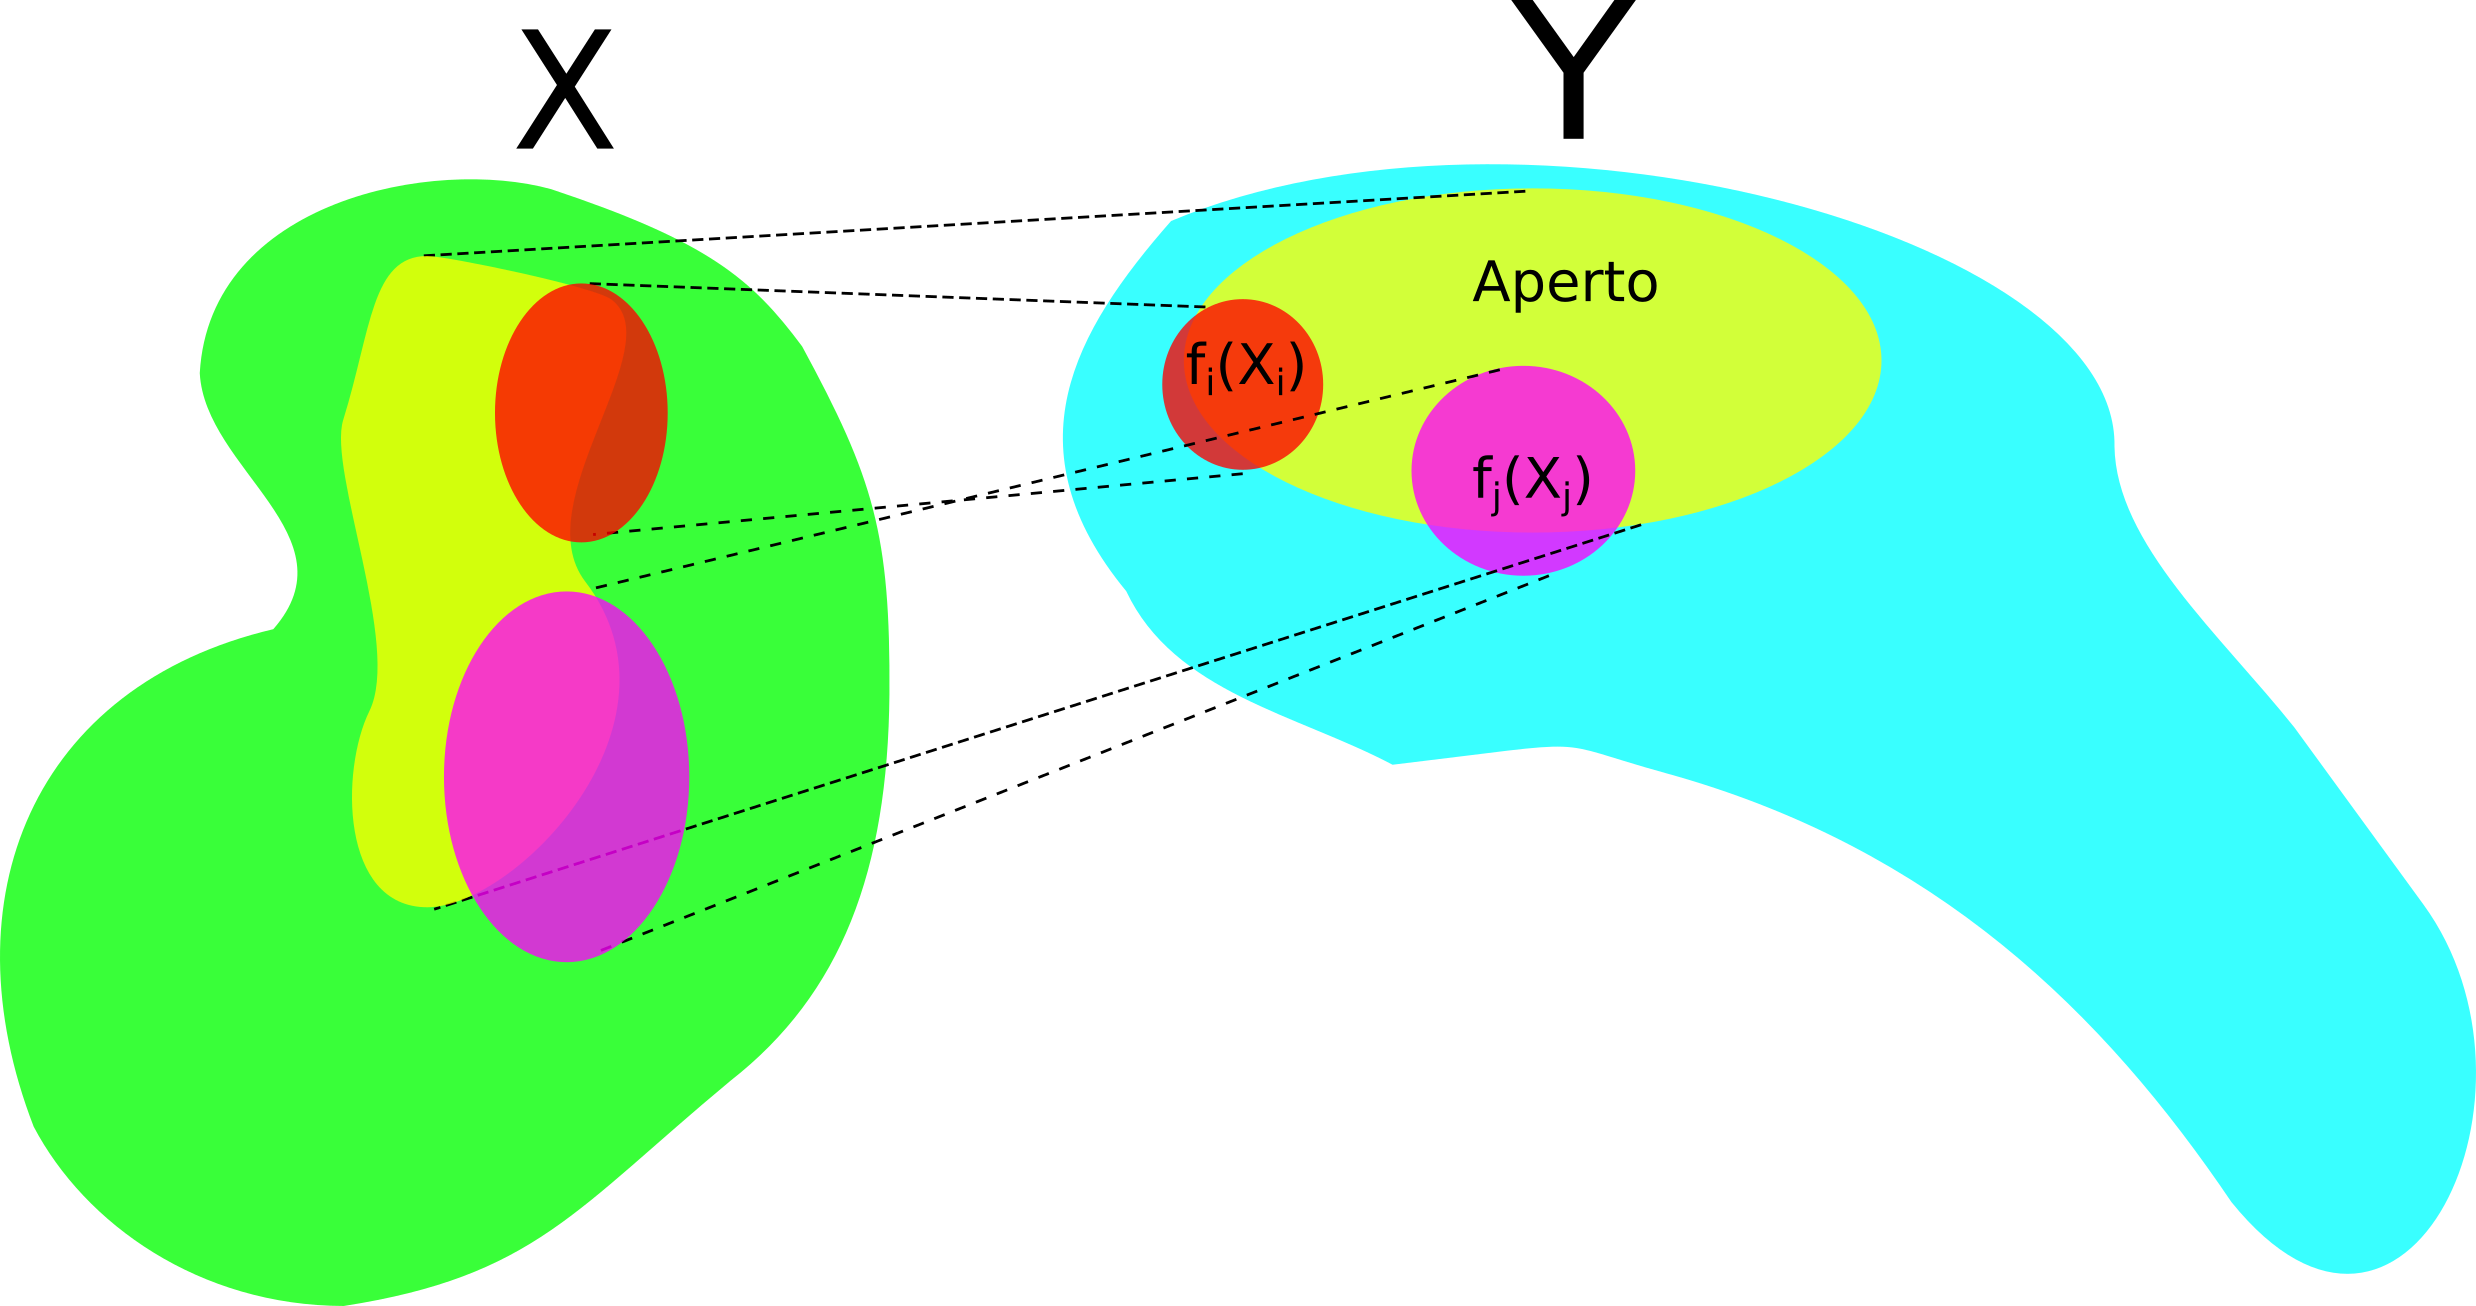
\includegraphics[width=0.6\linewidth]{images/topologia_generale/Coomology_exercises_figure}
		\caption{un'immagine del caso generico per convincersi}
		\label{fig:coomologyexercisesfigure}
	\end{figure}
	Devo solo dimostrare che la funzione $f$ globale è continua.
	Sia $A$ aperto in $\xi$. Allora considero $f^{-1}(A)$. Per la definizione di $f$ e siccome potrebbe essere che una parte di $A \cap \image{f_j} \neq \varnothing$ e $A \cap \image{f_i} \neq \varnothing$, prendo tutte quelle funzioni la cui immagine contiene punti di $A$. Allora vale 
	\begin{equation*}
		f^{-1}(A) = \bigcup_{i} f_i^{-1}(A) 
	\end{equation*}
	ma poiché le funzioni $f_i$ sono continue negli $X_i$, portando la proprietà a livello globale ottengo che $f^{-1}(A) = X_i \cap A_i'$ per degli $A' \in \tau$. Dunque 
	\begin{equation*}
		f^{-1}(A) = \bigcup_{i} f_i^{-1}(A) = \bigcup_{i} X_i \cap A_i' 
	\end{equation*}
	ma $X_i, A'_i \in \tau$ quindi la loro intersezione è ancora un aperto, inoltre l'intersezione qualsiasi di aperti è un aperto. Segue che $f^{-1}(A)$ è aperto e dunque $f$ continua.
\end{proof}

\newpage



\subsection{\textcolor{TopGener}{\textbf{Il prodotto topologico finito}}}



In questa sezione si userà spesso la notazione 
\begin{equation*}
(X_1, \tau_1)
\end{equation*}
\begin{equation*}
(X_2, \tau_2)
\end{equation*}
\begin{equation*}
(X_1 \times X_2, \tau = \left\langle\tau_1 \times \tau_2 \right\rangle)
\end{equation*}
per indicare tre spazi topologici. L'ultimo in particolare è il prodotto di due spazi topologici che adesso definiremo.
%todo: controlla se ti piace come sono allineati, io li preferisco centrati ma cambia poco per me, so che preferisci avere... 
%todo: ... tutto allineato di solito (mi dava fastidio che andasse a capo) (s)

\begin{definition}
	La topologia $\tau$ che viene generata dalla base $\tau_1 \times \tau_2$ è detta topologia prodotto su $X_1 \times X_2$. Inoltre $(X_1 \times X_2, \tau)$ è uno spazio topologico e si dice prodotto degli spazi topologici $(X_1, \tau_1), (X_2, \tau_2)$.
\end{definition}

\begin{remark}
	Per quanto ovvio, facciamo vedere che $\tau_1 \times \tau_2$ forma una base su $X_1 \times X_2$. \\ Per la Proposizione \ref{thr:sfi_generate_topology} un insieme è una base di $X_1 \times X_2$ se tale insieme copre $X_1 \times X_2$, ma questo è ovvio visto che $X_1 \times X_2 \in \tau_1 \times \tau_2$; e dati due elementi $A_1, A_2 \in \tau_1 \times \tau_2$ allora la loro intersezione 
	\begin{equation*}
	A_1 \cap A_2 = B_{1,1} \times B_{2,1} \cap B_{2,1} \times B_{2,2} = B_{1,1}\cap B_{2,1} \times B_{1,2} \cap B_{2,2}
	\end{equation*}
	dove ogni $B_{j,i} \in \tau_j \cap A_i$ per cui sono ancora elementi di $\tau_1 \times \tau_2$. Pertanto è una base ed identifica un unica topologia.
\end{remark}

\begin{example}
	Si consideri $(\R^2, \tau^2_{\text{euclidea}})$, allora questo sarà omeomorfo a $(\R, \tau) \times (\R, \tau)$? \\ Se la risposta fosse negativa non avrebbe senso parlare di prodotti di topologie, pertanto dobbiamo arrivare ad una risposta positiva. 
	In senso geometrico mi basta dimostrare la finezza tra le due topologie, quindi sceglierò la base più comoda per i miei scopi:
	\begin{itemize}
		\item $\tau'$ topologia risultante dal prodotto topologico (topologia prodotto), in $\mathbb{R}^2$ gli elementi della topologia avranno \enquote{la forma di rettangoli} (per capire la motivazione basti pensare a come funziona un prodotto cartesiano)
		\item $\tau$ topologia naturale di $\mathbb{R}^2$, noto che lo spazio è metrizzabile con la distanza euclidea
	\end{itemize}
	\textbf{$\tau'$ più fine di $\tau$}\\ In sostanza devo mostrare che ogni elemento della topologia naturale si può scrivere come \enquote{unione di rettangoli aperti}, questo è elementare: intuitivamente perché dentro ogni palla aperta è possibile prendere un rettangolo totalmente contenuto nella palla aperta. Più rigorosamente prendo $r$ raggio della palla aperta, $x$ tra $0$ ed $r$ (escluso) ed il quadrato aperto di base $r-x$: il quadrato è totalmente incluso nella palla aperta e per unione di questi quadrati posso ottenere la palla stessa. \\ \\
	\textbf{$\tau$ più fine di $\tau'$}\\ Come sopra, devo mostrare che ogni rettangolo si può scrivere come unione di palle aperte. Trovato il modo di incastrare la palla dentro il rettangolo aperto questo è immediato, basta usare il fatto che lo spazio sia metrizzabile. \\ \\
	In generale si può dimostrare che $\tau^n = \underset{n-volte}{\underbrace{\tau \times \dots \times \tau}}$, dove $\tau$ è la topologia euclidea. 
\end{example}

\begin{theorem}
	Sia $\mathcal{B}_1$ base di $\tau_1$ e $\mathcal{B}_2$ base di $\tau_2$, allora
	\begin{equation*}
		\mathcal{B}_1 \times \mathcal{B}_2 \coloneqq \left\{B_1 \times B_2 \in 2^{\mathcal{B}_1 \times \mathcal{B}_2} \,\middle|\, B_1 \in \mathcal{B}_1, \; B_2 \in \mathcal{B}_2\right\}
	\end{equation*}
	forma una base della topologia $\tau$ (ovvero il generato del prodotto delle topologie).
\end{theorem}
\begin{proof}
	Devo far vedere che se $A \in \tau$ allora è generato dalla base $\mathcal{B}_1 \times \mathcal{B}_2$. \\ Se $A \in \tau$, la topologia è generata dalla base $\tau_1 \times \tau_2$. Per cui $A = \bigcup_{i \in I} A_{1,i} \times A_{2,i}$, dove $A_{1,i} \in \tau_1$ e $A_{2.i} \in \tau_2$ per ogni $i \in I$. Ma ogni $A_{1, i} = \bigcup_{B \in \mathcal{B}_{1,i}'} B$, dove $\mathcal{B}_{1,i}' \subset \mathcal{B}_1$ e analogamente per $A_{2,i}$. Sostituendo si ottiene
	\begin{equation*}
		A = \bigcup_{i \in I} A_{1,i} \times A_{2,i} = \bigcup_{i \in I} \bigcup_{B \in \mathcal{B}_{1,i}'} B \times \bigcup_{B \in \mathcal{B}_{2,i}'} B = \bigcup_{\substack{i \in I \\ B_1 \in \mathcal{B}'_{1,i} \\ B_2 \in \mathcal{B}'_{2,i}}} B_1 \times B_2
	\end{equation*}
	Notare che $B_1 \times B_2$ indica tutti i possibili prodotti tra gli insiemi nelle rispettive famiglie, $\mathcal{B}'_{1,i}$ e $\mathcal{B}'_{2,i}$, e questi sono sempre elementi di $\mathcal{B}_1 \times \mathcal{B}_2$ e la somma dipende solo da $I$, per cui genera $A$. \\
	
	Devo vedere anche che la topologia generata da $\mathcal{B}_1 \times \mathcal{B}_2$ non sia più fine di $\tau$. Per cui sia $A \in \left\langle \mathcal{B}_1 \times \mathcal{B}_2 \right\rangle$. Allora $A = \bigcup_{i \in I} B_{1,i} \times B_{2,i}$, mi basta considerare la proiezione di $A$ (che è una mappa aperta) per vedere che 
	\begin{equation*}
	\pi_1(A) = \bigcup_{i \in I} B_{1,i} = A_1 \in \tau_1
	\end{equation*}
	 e analogamente per $\tau_2$. \\ Per cui risulta che $A_1 \times A_2 = \pi_1(A) \times \pi_2(A) = A$.
\end{proof}


\begin{theorem}
	La topologia prodotto $\tau$ è la meno fine per cui le mappe $\morphism{\pi_i}{X_1\times X_2}{X_i}$ sono continue.
\end{theorem}
\begin{proof}
	La topologia prodotto rende palesemente le mappe continue, dobbiamo solo verificare che sia la più fine. \\
	Suppongo esista una topologia meno fine di $\tau$ che chiamerò $\tau'$. Allora $\pi_1$ è continua e quindi contiene almeno tutti gli aperti della forma $\pi^{-1}_1(A_1) \times \pi^{-1}_2(A_2)$ dove $A_i$ aperto in $\tau_i$. Ma questi aperti sono esattamente gli aperti della base che genera $\tau$, pertanto $\tau \subset \tau'$.
\end{proof}

\begin{theorem}
	Le mappe $\morphism{\pi_i}{X_1\times X_2}{X_i}$ sono aperte (dove $i \in \left\{1,2\right\}$). 
\end{theorem}
\begin{proof}
	Si consideri $\pi_1(A)$ dove $A \in \tau$. Allora $A = \bigcup_{i \in I} A_{1,i} \times A_{2,i}$, per cui $\pi(A) = \pi(\bigcup_{i \in I} A_{1,i} \times A_{2,i}) = \bigcup_{i\in I} \pi_1 (A_{1,i} \times A_{2,i}) = \bigcup_{i \in I} A_{1,i}$. Poiché ogni $A_{1,i} \in \tau_1$ segue che anche la loro unione lo è. Analogamente si dimostra per la proiezione $\pi_2$.
\end{proof}

\begin{theorem}
	Siano $S_1 \subset X_1, S_2, \subset X_2$; il prodotto di sotto topologie si comporta bene, ovvero
	\begin{equation*}
		\left\langle \tau_1 \times \tau_2 \right\rangle|_{S_1 \times S_2} = \left\langle \tau_1|_{S_1} \times \tau_2|_{S_2} \right\rangle 
	\end{equation*}
\end{theorem}
\begin{proof}
	Spezzo la dimostrazione nelle due inclusioni. Dimostro come primo caso $	\left\langle \tau_1 \times \tau_2 \right\rangle|_{S_1 \times S_2} \subset \left\langle \tau_1|_{S_1} \times \tau_2|_{S_2} \right\rangle$. \\ Quindi sia $A \in \left\langle \tau_1 \times \tau_2 \right\rangle|_{S_1 \times S_2}$ allora $A = \left( \bigcup_{i \in I} A_{1,i} \times A_{2,i} \right) \cap S_1 \times S_2$, per cui posso distribuire l'intersezione su tutti gli elementi dell'unione:
	\begin{equation*}
		\left( \bigcup_{i \in I} A_{1,i} \times A_{2,i} \right) \cap S_1 \times S_2 = \bigcup_{i \in I} (A_{1,i} \cap S_1) \times (A_{2,i} \cap S_2)
	\end{equation*}
	per il Teorema \ref{thr:proprieties_induced_top} per ogni $i \in I$, $(A_{1,i} \cap S_1) \times (A_{2,i} \cap S_2) \in \tau_1|_{S_1} \times \tau_2|_{S_2}$, ovvero $A \in \left\langle \tau_1|_{S_1} \times \tau_2|_{S_2} \right\rangle$. \\ \\ Come si può notare le implicazioni fatte sopra valgono anche nel verso opposto, per cui è dimostrata la tesi.
\end{proof}

\begin{theorem}
	Gli intorni si \emph{\enquote{comportano bene}} rispetto al prodotto topologico. In questo modo voglio dire che:
	\begin{enumerate}
		\item Sia $(x_1, x_2) \in X_1\times X_2$, allora $P \in \mathcal{N}_\tau((x_1,x_2))$ se e solo se esistono $U_1 \in \mathcal{N}_{\tau_1}(x_1)$ e $U_2 \in \mathcal{N}_{\tau_2}(x_2)$ tali che $U_1\times U_2 \subset P$.
		\item Siano $(x_1, x_2) \in X_1\times X_2$, $\mathcal{V}_1(x_1)$ e $\mathcal{V}_2(x_2)$ rispettivamente un sistema fondamentale di intorni di $x_1$ in $\tau_1$ e di $x_2$ in $\tau_2$; allora $\mathcal{V}_1(x_1) \times \mathcal{V}_2(x_2)$ è un sistema fondamentale di intorni di $(x_1, x_2)$ nella topologia $\tau = \left\langle \tau_1 \times \tau_2 \right\rangle$.
	\end{enumerate}	
\end{theorem}
\begin{proof} \textbf{Punto 1:}
	\begin{enumerate}
		\item[$\Leftarrow$] Abbastanza ovvio. Per definizione di intorno su $U_1$ esiste $A_1 \in \tau_1$ tale che $A_1 \subset U_1$, ed un discorso analogo vale su $\tau_2$. Allora $A_1 \times A_2 \in \tau$ per definizione, inoltre ho che 
		\begin{equation*}
			A_1 \times A_2 \subset U_1 \times U_2 \subset P
		\end{equation*}
		per cui $P$ è un intorno in $\tau$.
		\item[$\Rightarrow$] Per definizione di intorno questo vuol dire che esiste $A \subset P$ tale che $A \in \tau$. Allora $A = \bigcup_{i \in I} A_{1,i} \times A_{2,i}$, prendo $A_{1,i_0}, A_{2,i_0}$ tali da contenere rispettivamente $x_1, x_2$. Devo dimostrare che $A_{1,i_0}$ è un intorno di $x_1$ in $\tau_1$, ma è ovvio poiché $A_{1,i_0} \in \tau_1$. Analogo discorso su $A_{2,i_0}$. Ho dunque trovato un intorno in $\tau_1$ e uno in $\tau_2$ tali che il loro prodotto sta in $P$ (poiché il loro prodotto sta addirittura in $A \subset P$).
	\end{enumerate}
\end{proof}
\begin{proof} \textbf{Punto 2:} Abbiamo provato il risultato per gli intorni. \\ Sia $x=(x_1,x_2)$ fissato, siano
	\begin{itemize}
		\item $U_1$ intorno in $X_1$ di $x_1$, per ipotesi esiste un $V_1$ appartenente al sistema fondamentale di intorni con $x_1 \in V_1 \subset U_1$
		\item $U_2$ intorno in $X_2$ di $x_2$, per ipotesi esiste un $V_2$ appartenente al sistema fondamentale di intorni con $x_2 \in V_2 \subset U_2$
	\end{itemize}
	Siccome è ben noto (l'abbiamo provato) che $U$ intorno di $x$ si può comporre come
	\begin{equation*}
	U =U_{1}\times U_{2}
	\end{equation*}
	con $U_{i}$ intorni degli $x_i$, otteniamo subito la tesi.
	\begin{equation*}
	x=(x_1,x_2) \in V_1 \times V_2 \subset U_1 \times U_2
	\end{equation*}
	 Quindi il prodotto di un sistema fondamentale di intorni è sistema fondamentale di intorni del prodotto.
\end{proof}

\begin{theorem}
	Siano $S_1 \subset X_1, S_2 \subset X_2$, allora valgono le seguenti formule
	\begin{align*}
		\overline{S_1\times S_2}^{\tau} & = \overline{S_1}^{\tau_1} \times \overline{S_2}^{\tau_2} \\
		Int(S_1 \times S_2) & = Int(S_1) \times Int(S_2)\\
		Fr(S_1 \times S_2) &= (Fr(S_1) \times \overline{S_2}) \cup (\overline{S_1} \times Fr(S_2))
	\end{align*}
\end{theorem}
\begin{proof}[Dimostrazione equazione 1]
	Uso il fatto che un punto $x \in \overline{S_1\times S_2}^\tau$ se e solo se $x$ è aderente a $S_1 \times S_2$ in $\tau$. Fisso dunque un $(x_1, x_2) \in \overline{S_1\times S_2}^\tau$ e dei sistemi fondamentali di intorni $\mathcal{V}_{\tau_1}(x_1), \mathcal{V}_{\tau_2}(x_2)$.\\
	L'aderenza per definizione indica che esiste un sistema fondamentale di intorni $\mathcal{V}_\tau(x) = \mathcal{V}_{\tau_1}(x_1) \times \mathcal{V}_{\tau_2}(x_2)$ tale che per ogni $V \in \mathcal{V}_\tau(x)$ vale $V \cap S_1 \times S_2 \neq \varnothing$. Usando la definizione data di $\mathcal{V}_\tau(x)$ posso riscrivere come per ogni $V_1 \in \mathcal{V}_{\tau_1}(x_1), V_2 \in \mathcal{V}_{\tau_2}(x_2)$ tali che $V_1 \times V_2 \cap S_1 \times S_2 \neq \varnothing$. \\ 
	Applicando un po' di leggi insiemistiche diventa $V_1 \cap S_1 \times V_2 \cap S_2 \neq \varnothing$, ovvero $V_1 \cap S_1 \neq \varnothing$ e $V_2 \cap S_2\neq \varnothing$, per cui dev'essere che $x_1$ sia aderente a $S_1$ secondo $\tau_1$; ed analogamente per $x_2$. 
\end{proof}
\begin{proof}[Dimostrazione equazione 2]
		\begin{equation*}
		Int(S \times T) = Int(S) \times Int(T)
		\end{equation*}
	\begin{itemize}
		\item[($\subset$)] Sia $x \in Int(S \times T)$, questo vuol dire che esiste un intorno di $x$ totalmente contenuto in $S \times T$. Sia $A$ tale intorno (posso supporlo aperto a meno di restrizione), per proprietà viste posso decomporlo come 
		\begin{equation*}
		x \in A = A_1 \times A_2 
		\end{equation*}
		Ma questo vuol dire che le due componenti di $x$ hanno intorni rispettivamente dentro $S$ e dentro $T$.
		\item[($\supset$)] Sia $x \in Int(S) \times Int(T)$, questo vuol dire che le due componenti di $x$ hanno intorni (aperti a meno di restrizione) totalmente contenuti in $S$ e $T$, procedendo come prima ottengo subito la tesi.
	\end{itemize}
\end{proof}
\begin{proof}[Dimostrazione equazione 3]
	Considero, analogamente a quanto fatto per dimostrare la prima equazione, $(x_1,x_2) \in Fr(S_1 \times S_2)$. Fisso un sistema fondamentale di intorni su $S_1$ e $S_2$. Per cui se $x \in Fr(S_1 \times S_2)$, allora $V \cap S_1 \times S_2\neq \varnothing$ e $V \not\subset S_1 \times S_2$. Sostituendo la decomposizione per sistemi fondamentali di intorni $V_1 \times V_2 \cap S_1 \times S_2 = V_1 \cap V_2 \times S_1 \cap S_2\neq \varnothing$ per cui $V_1 \cap S_1 \neq \varnothing$ e $V_2 \cap S_2 \neq \varnothing$. Inoltre dalla condizione $V \not\subset S_1 \times S_2$ si ottengono le condizioni \textit{esclusive}:
	\begin{enumerate}
		\item $V_1 \subset S_1 \land V_2 \not\subset S_2$
		\item $V_1 \not\subset S_1 \land V_2 \subset S_2$
		\item $V_1 \not\subset S_1 \land V_2 \not\subset S_2$
	\end{enumerate}
	Unendo tutte le condizioni si ottiene la tesi. 
\end{proof}

\begin{theorem}[Proprietà universale del prodotto topologico]
	Sia data 
	\begin{equation*}
	\morphism{f}{(Y, \xi)}{(X_1 \times X_2, \tau)}
	\end{equation*}
	una applicazione su spazi topologici e siano $\pi_1,\pi_2$ le proiezioni canoniche dal prodotto topologico. Allora $f_i = \pi_i \circ f$ si dicono componenti di $f$ e vale l'equivalenza delle seguenti affermazioni:
	\begin{enumerate}
		\item $f$ è continua
		\item $f_i$ sono continue per $i \in \left\{1,2\right\}$
	\end{enumerate}
	\begin{equation*}
	\begin{tikzcd}[column sep=0.7em]
	& (Y, \xi) \arrow[swap]{d}{f} \arrow[swap]{ddl}{f_1} \arrow{ddr}{f_2} & \\
	& (X_1 \times X_2, \tau) \arrow[swap]{dr}{\pi_2} \arrow{dl}{\pi_1} & \\
	(X_1, \tau_1) &  & (X_2, \tau_2)\\
	\end{tikzcd}
	\end{equation*}

\end{theorem}
\begin{proof} \
	\begin{enumerate}
		\item[$\Leftarrow$] Se $f$ continua allora $\pi_1 \circ f$ è continua, perché composizione di funzioni continue, analogamente per $\pi_2 \circ f$.
		\item[$\Rightarrow$] Questa è la proprietà meno ovvia e la più importante del teorema. \\ Se le componenti $f_1, f_2$ sono continue. Allora si prenda un aperto $A \in \tau$, e si prenda la sua controimmagine attraverso $f$. È ovvio che dati $A_{1}, A_{2}$ aperti rispettivamente in $\tau_1, \tau_2$ vale
		\begin{align*}
		f^{-1}(A) & = f^{-1}\left(\bigcup_i A_{1,i} \times A_{2,i}\right)=\bigcup_i f^{-1}\left(A_{1,i} \times A_{2,i}\right)\\
		& = \bigcup_i f^{-1}\left\{y \in Y \text{ con } f(y) \in A_{1,i} \times A_{2,i}\right\}\\ 
		& = \bigcup_i f^{-1}\left\{y \in Y \text{ con } f_j(y) \in A_{j,i} \text{ per $j=1,2$}\right\}\\
		& = \bigcup_i \left(f_1^{-1}(A_{1,i})\cap f_2^{-1}(A_{2,i})\right)
		\end{align*}
		Siccome non abbiamo ancora usato l'ipotesi, è arrivato il momento di usarla. Infatti si vede che essendo $f_1, f_2$ continue, la loro controimmagine di aperti è aperta. Da cui ho anche $f^{-1}(A_{1,i} \times A_{2,i})$ aperto; $f$ è continua. 
	\end{enumerate}
\end{proof}
%\begin{proof}[Dimostrazione utilizzando le proprietà degli s.f.i.]
	% TODO: `? CASUAL': Una dimostrazione alternativa, di un teorema già dimostrato (g)
	%todo: non penso sia necessario, se vuoi provare falla (s)
%\end{proof}
La proprietà universale del prodotto topologico è molto utile in applicazioni pratiche, inoltre notiamo che è possibile dimostrarla sfruttando le proprietà dei sistemi fondamentali di intorni.
\begin{theorem}
	Sia $\morphism{g}{(X_1 \times X_2, \tau)}{(Y, \xi)}$. Fissato un $(x_1, x_2) \in X_1 \times X_2$ le seguenti sono equivalenti.
	\begin{enumerate}
		\item $g$ è continua in $(x_1, x_2)$
		\item per ogni intorno $U \in \mathcal{N}_\xi(g(x_1,x_2)))$ esistono $V_1 \in \mathcal{V}_1(x_1)$ e $V_2 \in \mathcal{V}_2(x_2)$ tali che $g(V_1 \times V_2) \subset U$
	\end{enumerate}
\end{theorem}
\begin{proof}
	Se $g$ è continua in $x$ allora per ogni intorno $V$ di $g(x)$ esisterà un intorno $N$ di $x$ tale che $g(N) \subset V$. Poiché $N$ è un intorno nella topologia prodotto allora esistono $N_1, N_2$ rispettivamente intorni di $x_1, x_2$ dove $x = (x_1, x_2)$. Ovvero la tesi.\\ \\
	Al contrario, fissiamo $V$ intorno di $g(x)$, allora devo dimostrare che $g^{-1}(V)$ è ancora un intorno di $x$, ma questo è ovvio dato che esistono $N_1, N_2$ tali che $g(N_1 \times N_2) \subset g(g^{-1}(V)) \subset V$ e quindi $N_1 \times N_2 \subset g^{-1}(V)$. 
\end{proof}
\paragraph{Estendere i risultati per $n > 2$} \ \\ \\
Possiamo notare che in generale i teoremi dimostrati per $n=2$, ovvero $X=X_1 \times X_2$, valgono anche per il prodotto topologico di $n \in \N$ spazi topologici; infatti basta procedere per induzione. \\ Il vero problema è dimostrare che $X_1 \times X_2 \times \dots \times X_n \simeq X_1 \times (X_2 \times \dots \times X_n)$ e così via, cioè dimostrare che il prodotto di topologie è un operatore associativo nella categoria degli spazi topologici. 

\begin{theorem}
	Le topologie con l'operazione di prodotto formano un monoide commutativo su $Top/\sim$, dove $X\sim Y$ se e solo se $X$ è omeomorfo $Y$.
\end{theorem}
\begin{proof} \
	\begin{enumerate}
		\item \textit{Associatività} \\Ovvia.
		\item \textit{Commutatività} \\Basta definire la mappa $\morphism{f}{X\times Y}{Y \times X}$, con $f(x,y) = (y,x)$. La mappa così definita è continua, biettiva e aperta. Per cui la proprietà commutativa vale.
		\item L'identità è il singoletto $\left\{p\right\}$ con la topologia qualsiasi (tanto è sempre la stessa). Quindi sia $(X, \tau)$ uno spazio topologico. Definisco la mappa $\morphism{f}{(X, \tau)}{(X\times \left\{p\right\}, \tau')}$ nell'unico modo in cui è possibile definirla. La mappa è biettiva perché $f^{-1}(x, p) = x$ è la sua funzione inversa. È ovviamente continua perché $f^{-1}((A, \varnothing)) = \varnothing$, $f^{-1}((A, \left\{p\right\})= A$ perché $f$ biettiva. E analogamente si dimostra che è aperta. Pertanto è l'identità. 
	\end{enumerate}
\end{proof}



\subsection{\textcolor{TopGener}{\textbf{Topologie quozienti}}}



\begin{definition}[Topologia quoziente]
	Sia $(X, \tau)$ spazio topologico e $\morphism{f}{X}{Y}$ applicazione, con $Y \neq \varnothing$. Si dice\textbf{ topologia quoziente su $Y$ rispetto ad $f$}, oppure \textbf{topologia indotta da $f$ su $Y$}, la più fine topologia su $Y$ tale che $f$ è continua. 
\end{definition}

\begin{theorem}
	Sia $(X, \tau)$ spazio topologico e $\morphism{f}{X}{Y}$ applicazione e $Y \neq \varnothing$. Valgono le seguenti affermazioni.
	
	\marginpar{\textbf{\textcolor{TopGener}{La proprietà universale dei quozienti topologici:}} perché è interessante questa proprietà universale? La proprietà è addirittura fondamentale, perché permette di by-passare la topologia quoziente per verificare che una mappa è continua, senza dover lavorare sulla topologia quoziente stessa.}
	
	
	
	\begin{enumerate}
		\item La topologia quoziente su $Y$ rispetto a $f$ esiste ed è unica, inoltre denotandola come $\tau_f$ vale 
		\begin{equation*}
			\tau_f \coloneqq \left\{ A \in 2^Y \,\middle|\, f^{-1}(A) \in \tau \right\}
		\end{equation*}
		\item $C$ è chiuso in $\tau_f$ se e solo se $f^{-1}(C)$ è chiuso in $\tau$.
		\item La topologia quoziente rispetto ad $f$ è la topologia più fine che rende $f$ continua.
		\item \textbf{Proprietà universale degli  spazi quozienti:} Sotto le ipotesi precedenti, sia $f$ continua. Considerando il seguente diagramma 
		\begin{equation*}
		\begin{tikzcd}
		(X, \tau) \arrow[swap]{rd}{g\circ f} \arrow{r}{f} & (Y, \tau_f) \arrow{d}{g} \\
		& (Z, \mu) 
		\end{tikzcd}
		\end{equation*}
		$g$ è continua se e solo se $g \circ f$ è continua. 
	\end{enumerate}
\end{theorem}
\begin{proof} \
	\begin{enumerate}
		\item È ovviamente una topologia ed è la più fine. 
		\item La controimmagine commuta con il complementare. 
		\item Chiaramente, per come abbiamo definito la topologia quoziente.
		\item Se $g$ è continua è ovvio che $g \circ f$ è continua perché la composizione di funzioni continue è continua. \\ Se $f\circ g$ è continua, sia $A$ aperto  in arrivo rispetto a $g$, allora $g^{-1}(A)$ deve essere un aperto. 
		\begin{equation*}
		f^{-1}\left(g^{-1}(A)\right)=\left(g \circ f\right)^{-1}(A)
		\end{equation*}
		Siccome la composizione è continua per ipotesi allora ho ottenuto un aperto in partenza. Si noti l'importanza della topologia quoziente in $Y$.
	\end{enumerate}
\end{proof}

\begin{remark}
	Sia $\morphism{f}{(X, \tau)}{(Y, \tau_f)}$, se $f$ non è surgettiva allora $\exists y \in Y \setminus f(X)$; il singoletto $\left\{y\right\}$ è un aperto nella topologia $\tau_f$ poiché $f^{-1}(y) = \varnothing$.
\end{remark} 

\begin{definition}
	Sia $\morphism{f}{X}{Y}$ applicazione e sia $S \subset X$. Diciamo che $S$ è \textbf{saturo}\footnote{un'idea sul significato del termine è che essenzialmente la funzione \textit{divora} tutte le fibre di $S$ in modo tale che stiano in $S$ stesso.} rispetto a $f$ se $f^{-1}(f(S)) = S$.
\end{definition} 

\begin{remark}
	Possiamo caratterizzare $S$ sottospazio saturo rispetto ad $f$.
	\begin{equation*}
		S = f^{-1}f(S) = \bigcup_{x \in S} f^{-1}f(x)
	\end{equation*}
	ovvero se per ogni $x \in S$ abbiamo un'unica fibra in $S$. Ovvero $S$ contiene tutte le fibre di $f$ contenenti i suoi punti. 
\end{remark} 

\begin{remark}
	Se $f$ è iniettiva, allora ogni insieme è $f$-saturo, poiché $S = f^{-1}f(S)$.
\end{remark}

\begin{theorem}
	$\morphism{f}{X}{Y}$ applicazione e sia $S \subset X$. \\ $f^{-1}f(S)$ si dice \textbf{$f$-saturazione} di $S$. Si può dimostrare che 
	\begin{enumerate}
		\item $S \subset f^{-1}f(S)$
		\item $f^{-1}\left(f(S)\right)$ è il più piccolo insieme $f$-saturo contenente $S$.
	\end{enumerate}
\end{theorem}
\begin{proof}\
	\begin{enumerate}
		\item Ovvio. Volendo usare quanto detto nell'osservazione precedente
		\begin{equation*}
			S = \bigcup_{x\in S} \left\{x\right\} \subset \bigcup_{x \in S} f^{-1}f(x)
		\end{equation*}
		e l'uguaglianza vale solo se $S$ è saturo.
		\item È semplice vedere che
		\begin{equation*}
			f(f^{-1}(f(S))) = f(S) \Longrightarrow f^{-1}(f(f^{-1}(f(S)))) = f^{-1}(f(S))
		\end{equation*}
		poiché se $x \in f^{-1}(f(S))$ allora $f(x) \in f(S)$ per definizione (e viceversa), quindi la $f$-saturazione di $S$ è $f$-satura. Devo inoltre dimostrare che è la più piccola. Per cui sia $K$ $f$-saturo tale che $S \subset K \subset f^{-1}f(S)$. Applicando $f^{-1}f$ sulla precedente successione di inclusioni (dove per comodità di lettura abbiamo omesso le parentesi, per esempio $f \ g = f(g)$)
		\begin{equation*}
			f^{-1}f(S) \subset f^{-1}f(K) \overset{\text{è f-sat.}}{=} K \subset f^{-1}ff^{-1}f(S) = f^{-1}f(S) 
		\end{equation*}
		Ottengo che $K = f^{-1}f(S)$. Per cui la più piccola è necessariamente $f^{-1}f(S)$ 
	\end{enumerate}
\end{proof}

\subsection{\textcolor{TopGener}{\textbf{Quozienti con mappe surgettive}}}
La topologia quoziente può essere cattiva. Decisamente cattiva. \\
Costruire un modo più facile per studiarla è necessario per i casi peggiori e più contorti; possiamo provare a collegare le proprietà della topologia $\tau_f$ a quella di partenza $\tau$. \\ Uno strumento utile saranno le identificazioni.

\begin{lemma}
	Sia $\morphism{f}{X}{Y}$ applicazione surgettiva e $S \subset X$ $f$-saturo, allora 
	\begin{enumerate}
		\item $S^c$ è $f$-saturo 
		\item $f(S^c) = f(S)^c$
	\end{enumerate}
\end{lemma}
\begin{proof}
	Dimostro per prima cosa $f(S)^c = f(S^c)$. Data $f$ suriettiva allora 
	\begin{equation*}
		f(X) = f(S \cup S^c) = f(S) \cup f(S^c) = Y
	\end{equation*}
	e dunque $f(S^c) = Y \setminus f(S) = f(S)^c$. 
	Per la $f$-saturazione di $S$ ho che $S = f^{-1}f(S)$, dunque applicando il complementare ottengo immediatamente che 
	\begin{equation*}
	S^c = f^{-1}(f(S))^c = f^{-1}(f(S)^c) = f^{-1}(f(S^c))
	\end{equation*}
\end{proof}

\begin{theorem}
	Sia $(X, \tau)$ spazio topologico, $\morphism{f}{X}{Y}$ surgettiva ed $Y$ con $\tau_f$ allora vale 
	\begin{enumerate}
		\item $A \subset Y$ è un aperto in $\tau_f$ se e solo se esiste $Q \in \tau$ tale da essere $f$-saturo e che $f(Q) = A$. Dunque vale 
		\begin{equation*}
			\tau_f = \mathcal{A} = \left\{ A \in 2^Y \,\middle|\, A = f(S), \text{dove}\ S \in \tau, f^{-1}f(S) = S\right\}
		\end{equation*}
		\item $C \subset Y$ è un chiuso in $\tau_f$ se e solo se esiste $Q \subset X$ chiuso tale da essere $f$-saturo e che $f(Q) = C$.
	\end{enumerate}
\end{theorem}
\begin{proof} \
	\begin{enumerate}
			\item Sia $A \in \mathcal{A}$, allora esiste $S \in \tau$ tale da essere $f$-saturo. Per cui $f^{-1}(A) = f^{-1}(f(S)) \overset{\text{saturazione}}{=} S \in \tau$. Questo dimostra $\mathcal{A} \subset \tau_f$. Sia dunque $A \in \tau_f$ e $U = f^{-1}(A) \in \tau$, devo dimostrare che $U$ è $f$-saturo. 
			Dato che $f(f^{-1}(A)) = A$ per la surgettività di $f$   
			\begin{equation*}
				f^{-1}f(U) = f^{-1}(A) = U
			\end{equation*} 
			e dunque è anche $f$-saturo. Si evince che $\tau_f \subset \mathcal{A}$ e dunque anche che $\tau_f = \mathcal{A}$.
		\item Devo dimostrare che un chiuso in $\tau_f$ è sempre della forma $K = f(C)$ per $C$ $f$-saturo e $C$ chiuso in $\tau$. Quindi vale che $K^c = f(S)$ dove $S \in \tau$ e $f$-saturo. Quindi posso riscrivere $S = C^c$ dove $C$ chiuso in $\tau$. Per il precedente lemma ho dunque
		\begin{equation*}
			K^c = f(S) = f(C^c) \overset{\text{lem. prec.}}{=} f(C)^c
		\end{equation*}
		dove $C$ è un chiuso $f$-saturo. Ovvero per ogni $K$ chiuso in $\tau_f$, vale $K = f(C)$ per qualche $C$ chiuso in $\tau$ e $f$-saturo (e viceversa), cioè la tesi.
	\end{enumerate}
\end{proof}

\begin{definition}
	Una applicazione $\morphism{f}{(X,\tau)}{(Y, \xi)}$ tra spazi topologici è detta \textbf{identificazione} se è continua, surgettiva e $\xi = \tau_f$.
\end{definition}

\begin{theorem}[Caratterizzazione delle identificazioni]
	\label{crtident}
	Sia data una funzione $\morphism{f}{(X,\tau)}{(Y, \xi)}$ continua e surgettiva, allora le seguenti affermazioni sono equivalenti.
	\begin{enumerate}
		\item $f$ è un identificazione.
		\item Se $\forall A \subset Y$  tale che $f^{-1}(A) \in \tau$ allora $A \in \xi$.
		\item Se $\forall A \in \tau$ $A$ è $f$-saturo, $f(A) \in \xi$.
		\item Se $\forall C \subset X$ chiuso e $f$-saturo vale $f(C)$ chiuso in $\xi$.
	\end{enumerate}
\end{theorem}
\begin{proof}\
	\begin{enumerate}
		\item[$(1 \Leftrightarrow 2)$] $f$ identificazione se e solo se $\tau_f = \xi$ e abbiamo gratis che $\xi \subset \tau_f$ perché topologia più fine tale da render $f$ continua. Quindi bisogna dimostrare $\tau_f \subset \xi \Longleftrightarrow \forall A \subset Y$ tali che $f^{-1}(A) \in \tau \Rightarrow A \in \xi$. Per cui se vale $\tau_f \subset \xi$ è ovvio che per ogni $A$ con $f^{-1}(A) \in \tau$ si ha $A \in \tau_f \subset \xi$, e ho la tesi. Se invece vale $\forall A \subset Y$ tali che $f^{-1}(A) \in \tau \Rightarrow A \in \xi$ allora se prendo $A \in \tau_f$ allora dev'essere che $f^{-1}(A) \in \tau$ e per ipotesi vale anche che $A \in \xi$ quindi $\tau_f \subset \xi$. 
		\item[$(1 \Rightarrow 3)$] Fisso $U \in \tau$ tale da essere $f$-saturo, allora $f(U) \in \xi = \tau_f$, ma $\xi = \tau_f$ per ipotesi, ovvero si ottiene la tesi.
		\item[$(3 \Rightarrow 1)$] Se vale $f(U) \in \xi$ devo provare che $\xi = \tau_f$, ma $\xi \subset \tau_f$ è già dimostrata poiché $\tau_f$ è la topologia più fine per cui $f$ sia continua. Per cui fisso un $A \in \tau_f$. $A \in \tau_f \Leftrightarrow \exists U \in \tau$ e $f$-saturo, ma per ipotesi $f(U) \in \xi$, quindi $\tau_f \subset \xi \subset \tau_f$.
		\item[$(3\Leftrightarrow 4)$] Ovvio per teoremi precedenti.
	\end{enumerate}
\end{proof}


\begin{remark}[Studio delle identificazioni]
	Notare che le identificazioni non sono sempre applicazioni aperte, anche se sono aperte e chiuse rispetto a una classe di insiemi (ovvero quelli $f$-saturi). \\ Infatti possiamo definire una applicazione non aperta e non chiusa.\\ Sia data 
	\begin{equation*}
	\morphism{f}{(\R, \tau_{\text{euclidea}})}{(\left\{0,1\right\})}
	\end{equation*}
	con $f \coloneqq \mathcal{X}_{\left[0,2\right)}$ dove la $\mathcal{X}$ è la mappa caratteristica dell'insieme a pedice. 
	\begin{itemize}
		\item \textbf{Riconoscere la topologia quoziente} \\ $\tau_f$ in questo caso è la topologia banale, infatti $0$ non può essere un aperto, in quanto se lo fosse $f^{-1}(0) = \left[0, 2\right)^c$ che non  è né aperto né chiuso. Analogamente per il punto $1$ che non può essere aperto (e neanche chiuso). 
		\item \textbf{La mappa non è aperta} \\ $f((0,2)) = 1$, per cui non manda aperti in aperti.
		\item \textbf{La mappa non è chiusa} \\ $f(\left[0,1\right]) = 1$ e dunque non manda neanche chiusi in chiusi, eppure $f$ è una identificazione.
	\end{itemize}
\end{remark}

\begin{theorem}
	Sia $\morphism{f}{(X,\tau)}{(Y, \tau_f)}$ identificazione, allora valgono le seguenti affermazioni.
	\begin{enumerate}
		\item $f$ aperta se e solo se $\forall A \in \tau$ la sua $f$-saturazione $f^{-1}f(A) \in \tau$
		\item $f$ chiusa se e solo se $\forall C$ chiuso la sua $f$-saturazione $f^{-1}f(C)$ è un chiuso.
	\end{enumerate}
\end{theorem}
\begin{proof}
	Dimostro solo il primo caso, il secondo è equivalente al primo dato quanto visto fino ad ora. Se $f$ aperta allora $\forall A \in \tau$ risulta che $f(A)$ è aperta per ipotesi e $f^{-1}f(A)$ dev'essere ancora un aperto perché $f$ continua. Se invece vale che la $f$-saturazione di un aperto è ancora aperta, fisso $A \in \tau$ e voglio vedere che $f(A)$ è un aperto in $\tau_f$. Ma $f(A) \in \tau_f$ se e solo se esiste $S \in \tau$ e $f$-saturo tale che $f(S) = f(A)$. Basta scegliere $S = f^{-1}f(A)$, e sappiamo che appartiene a $\tau$; è $f$-saturo ed inoltre poiché $f$ suriettiva $f(S) = f(f^{-1}f(A)) = f(A)$. Pertanto $f$ è aperta. 
\end{proof}

\subsection{\textcolor{TopGener}{\textbf{Relazioni di equivalenza e spazi quozienti}}}
La nostra ricetta più raffinata sarà quella degli \textbf{spazi quozienti}. 

\begin{flushright}
	{\fontfamily{cmss}\selectfont
		\textit{\textcolor{TopGener}{\textbf{Spazi quozienti alla relazione di equivalenza}}}\\
		Tempo di preparazione: 10 minuti\\
		Difficoltà: media
	}
\end{flushright}

Per la preparazione si raccomanda di avere delle relazioni di equivalenza fresche a portata di mano. \\ \\
{\Large \textbf{Ingredienti:}} \\
\begin{enumerate}
	\item Un insieme non vuoto, $X$.
	\item Una relazione di equivalenza $R \subset X \times X$.
\end{enumerate}
Si raccomandano ingredienti di provenienza topologica certificata.
\\ \\ {\Large \textbf{Preparazione:}} \\ \\
Raccolti gli ingredienti, è bene controllarne le date di scadenza. Da qui in avanti la procedura diventa semplice, si \textit{passa a quoziente}. Ma come? \\ Si prenda $X$ e lo si mappi in $X / R$, ovvero l'insieme delle classi di equivalenza di $X$ in $R$. 

\begin{figure}[h]
	\centering
	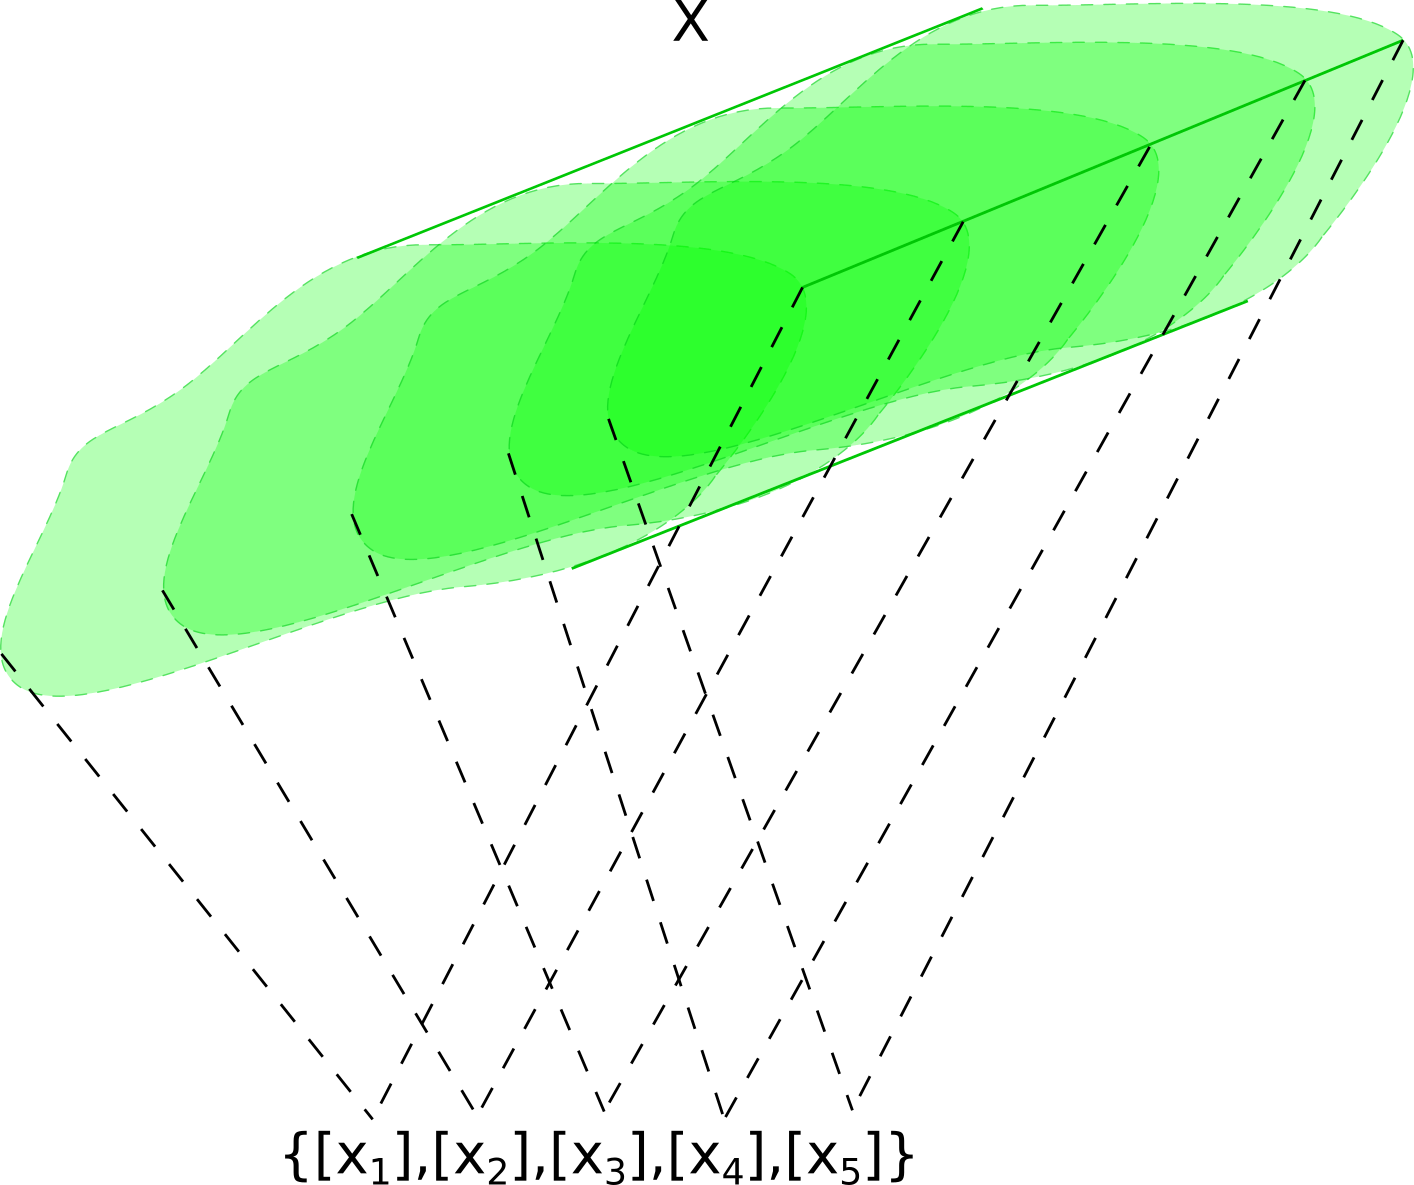
\includegraphics[width=0.5\linewidth]{images/topologia_generale/projection_quotient}
	\caption{proiezione della partizione di $X$ data dalla relazione $R$, oppure si possono vedere i sottoinsiemi verdi di $X$ come tutte le fibre di $f$ su un $X'$ proiettate in un punto da $\pi$}
	\label{fig:projectionquotient}
\end{figure}

Dopo aver cotto a fuoco lento per 2-3 minuti possiamo iniziare ad operare sui morfismi e costruire una mappa 
\begin{equation*}
\begin{tikzcd}[row sep = tiny]
	\pi  \colon &  X \arrow{r} & X/R \\
		 & x \arrow[mapsto]{r} & \left[x\right]_R
\end{tikzcd}
\end{equation*}
che è la \textbf{proiezione naturale} dell'insieme sul suo quoziente.\\  \\
 {\Large \textbf{Consigli:}} 
\\
\\
La proiezione naturale è sempre suriettiva  e si \enquote{comporta bene} (come si può vedere dalla figura).
\footnote{per questo si sono sempre studiate mappe suriettive nel capitolo precedente!}
 \\ \\ Utilizzando il procedimento canonico per la costruzione di topologie quozienti indotte da applicazioni sulla proiezione naturale, si ottiene quella che è detta \textbf{topologia quoziente di $\tau$ modulo $R$} e $(X/R, \tau_\pi)$ è detto lo spazio topologico quoziente di $(X,\tau)$ modulo $R$. 

\begin{lemma}
	\label{lem_qdom}
	Sia $\morphism{f}{(X, \tau)}{(X', \tau')}$ un'applicazione continua tra spazi topologici e siano $R, R'$ relazioni di equivalenza rispettivamente su $X, X'$. Vale $f(\left[x\right]_R) \subset \left[f(x)\right]_{R'}$ (equivale alla condizione $xRy \Rightarrow f(x)R'f(y)$) se e solo se esiste ed è unica una $g$ continua tale che il diagramma commuta.
	\begin{equation*}
	\begin{tikzcd}[row sep = 3em]
		(X, \tau) \arrow[swap]{d}{\pi} \arrow{r}{f} & (X', \tau') \arrow{d}{\pi'}\\
		(X/R, \tau_{X/R}) \arrow[swap]{r}{\exists! g} & (X'/R', \tau_{X'/R'})
	\end{tikzcd}
	\end{equation*} 	
	
\end{lemma}
\begin{proof}
	Se esiste $g$ per cui il diagramma commuta, stiamo praticamente dicendo 
	\begin{equation*}
		(\pi' \circ f)(x) = (g \circ \pi)(x) = (g \circ \pi)(y) = (\pi' \circ f)(y)
	\end{equation*}
	ma questa uguaglianza vale se e solo se $f(x) R' f(y)$, per cui ho la tesi.\\
	
	Dimostro l'esistenza di $g$ e la definisco come $g(\alpha) = (\pi' \circ f)(x_\alpha)$ dove $x_\alpha = \pi^{-1}\alpha$, ovvero $x_\alpha$ è un rappresentante della classe $\alpha$. Devo far vedere che sia ben definita, altrimenti non \textit{esiste}.
	Per cui considero anche un altro rappresentate della classe $\alpha$ e lo chiamo $x'_\alpha$. Affinché sia ben definita dev'essere che $g(\alpha) = \pi'f(x_\alpha) = \pi' f(x'_\alpha) = g(\alpha')$, ma questa condizione è vera per l'ipotesi. La continuità di $g$ è data dalla proprietà universale degli spazi quozienti, si consideri il seguente diagramma commutativo
	\begin{equation*}
		\begin{tikzcd}[row sep = 3em]
			(X,\tau) \arrow{d}{\pi} \arrow{rd}{\pi' \circ f} & \\
			(X/R, \tau_{X/R}) \arrow{r}{g} & (X'/R', \tau_{X'/R'})
		\end{tikzcd}
	\end{equation*}
	per cui $g$ è continua dato che $\pi' \circ f$ è continua.
\end{proof}

\begin{theorem}
	Sia  $\morphism{f}{X}{X'}$ una applicazione continua e surgettiva, possiamo definire la relazione di equivalenza $R_f$ sull'insieme $X$ ponendo la relazione $xR_fy \Leftrightarrow f(x) = f(y)$. Allora 
	\begin{enumerate}
		\item esiste ed è unica $\morphism{g}{X/R_f}{X'}$ biettiva e continua.
		\item $g$ è un omeomorfismo se e solo se $f$ è un identificazione.
	\end{enumerate}
\end{theorem}
\begin{proof}
	Basta applicare il Lemma \ref{lem_qdom} sul seguente diagramma
	\begin{equation*}
	\begin{tikzcd}[row sep = 3em]
		(X, \tau) \arrow[swap]{d}{\pi} \arrow{r}{f} & (X', \tau') \arrow{d}{\pi' = \operatorname{Id}}\\
		(X/R_f, \tau_{X/R_f}) \arrow[swap]{r}{\exists! g} & (X'/U', \tau_{X'/U'})
	\end{tikzcd}	
	\end{equation*}
	dove la relazione $U'$ su $X'$ è definita come $xU'y \Leftrightarrow x = y$, per cui la proiezione $\pi'$ non è nient'altro che l'identità. \\ Allora $(X'/U', \tau_{X'/U'}) = (X', \tau')$, inoltre il seguente diagramma commuta. 
	\begin{equation*}
	\begin{tikzcd}[row sep = 3em]
		(X, \tau) \arrow[swap]{d}{\pi} \arrow{r}{f} & (X', \tau') \\
		(X/R_f, \tau_{X/R_f}) \arrow[swap]{ru}{\exists! g} &
	\end{tikzcd}	
	\end{equation*}
	
	Per la commutatività del diagramma si ottiene senza fatica che $f = g \circ \pi$, e quindi dev'essere che se $f$ è suriettiva anche $g$ lo è. Inoltre $g$ è anche iniettiva: siano $\left[x\right] \neq \left[y\right]$, allora 
	\begin{equation*}
		f \circ \pi^{-1} (\left[x\right]) = g(\left[x\right]) \neq g(\left[y\right]) = f \circ \pi^{-1}(\left[y\right])
	\end{equation*}	
	poiché ogni controimmagine di una classe $\pi^{-1}(\left[x\right])$ sono tutti quegli $x_i \in X$ tali che $f(x_1) = f(x_2) = \dots = f(x_i)$. Dunque è anche iniettiva e risulta essere biettiva.\\
	
	Dimostro il secondo punto del teorema, per cui separo i due casi
	\begin{enumerate}
		\item[$(\Leftarrow)$] Sia $f$ identificazione Notare che abbiamo già che $g$ continua e biettiva, ci manca da dimostrare che $g$ aperta. \\ Sia $A \in \tau_{X/R_f}$ allora $\pi^{-1}(A) \in \tau$ ed è $f$-saturo. Allora $f(\pi^{-1}(A)) \in \tau_f$ e poiché $f = g \circ \pi$ risulta 
		\begin{equation*}
			 \tau_f \ni f(\pi^{-1}(A)) = g ((\pi \circ \pi^{-1})(A)) = g(A)
		\end{equation*}
		quindi $g$ è aperta e un omeomorfismo.
		\item[$(\Rightarrow)$] Poniamo $g$ omeomorfismo. Dobbiamo dimostrare che $f$ è un identificazione; sappiamo già che $f$ suriettiva e continua, quindi dobbiamo dimostrare l'uguaglianza delle  topologie in arrivo. \\ Per questo possiamo scegliere una delle caratterizzazioni date dal Teorema \ref{crtident}. In particolare se riusciamo a dimostrare che per ogni $A' \in 2^X$ tale che $f^{-1}(A') \in \tau$ allora $A' \in \tau'$, abbiamo vinto. Fisso un $A'$ tale che $f^{-1}(A') \in \tau$. Ma questo è $\pi$-saturo, quindi vale che $\pi f^{-1} (A') \in \tau_{X/R_f}$, inoltre grazie al fatto che $g$ è un omeomorfismo possiamo portare in avanti l'aperto senza problemi
		\begin{equation*}
			\tau' \ni g\pi (f^{-1}(A')) = ff^{-1}(A') \overset{f \; \text{surg.}}{=} A' 
		\end{equation*}
		che è quanto si voleva dimostrare.
	\end{enumerate}
\end{proof}

I seguenti corollari sono decisamente simili ed indicano la stessa cosa, ma in modi distinti e di diversa utilità pratica. 

\begin{corollary}
	Se $\morphism{f}{(X,\tau)}{(X',\tau')}$ è una identificazione, allora $(X/R_f, \tau_{R_f})$ è omeomorfo a $(X', \tau')$. 
\end{corollary}

\begin{corollary}
	Sia $(X,\tau)$ spazio topologico, sia $R$ relazione di equivalenza su $X$, $\morphism{\pi}{(X,\tau)}{(X/R, \tau_{X/R})}$ sua proiezione naturale e $(X', \tau')$ un altro spazio topologico. \\ Supponiamo esista $\morphism{f}{(X,\tau)}{(X',\tau')}$ identificazione tale che $f^{-1}f(x) = \left[x\right]_R$ per ogni $x \in X$, allora $X/R \simeq X'$. \\ \\ A livello intuitivo la richiesta $f^{-1}f(x) = \left[x\right]_R$ richiede che la funzione \enquote{rispetti le fibre} della relazione di equivalenza.
\end{corollary}



\section{Gruppi topologici}
\subsection{\textcolor{TopGener}{\textbf{L'operatore di gruppo}}}

Finalmente è giunto il momento di portare ad un livello superiore la nostra trattazione. I gruppi sono ubiquitari in matematica, e si presentano in varie forme in topologia i.e. gruppo fondamentale, gruppi di omologia, etc. In particolare l'argomento trattato ora, per quanto `fuori dal contesto' generale, si ricollega a costruzioni utili nella teoria dei rivestimenti e rivestimenti universali (argomenti profondi che avranno collegamenti anche con la teoria di Galois, si veda etalé homology).  


\begin{definition}
	Sia $(X, \tau)$ uno spazio topologico con $\cdot \colon X \times X \rightarrow X$ un operatore di gruppo su $X$. \\ Allora è un gruppo topologico se $x \cdot y^{-1}$ è una funzione continua.
\end{definition}

\begin{example} \
\begin{enumerate}
	\item $\R$ con la topologia euclidea e l'addizione è un gruppo topologico.
	\item $\Z, \Q$ sono due sottogruppi normali di $\R$ rispetto all'addizione. 
	\item $\operatorname{GL}_n(\R)$ e i suoi sottogruppi sono gruppi topologici sconnessi rispetto al prodotto tra matrici.
\end{enumerate}
\end{example}

